
%%
\documentclass{mcmthesis}
\mcmsetup{CTeX = false,   % 使用 CTeX 套装时,设置为 true
        tcn = 2212229, problem = A,
        sheet = true, titleinsheet = true, keywordsinsheet = true, titlepage = true, abstract = true}
\usepackage{newtxtext}%\usepackage{palatino}
\usepackage{lipsum}
\usepackage[numbers]{natbib}
\usepackage{amsmath}
\usepackage{float}
\usepackage{indentfirst}
\usepackage{setspace}
\usepackage{subfigure}
\usepackage{tocloft}
% \usepackage{ctex}
\title{Bicycle Time Trial Strategy Based on Power Profile}
% \author{\small QIU Xiaoyu, XU Shaojun, ZHU Shaoting}
%   {
\includegraphics[width=7cm]{mcmthesis-logo}}}
\date{\today}
\begin{document}
% 记住一定要少出现  we
\begin{abstract}
\par
Strategy plays an important role in cycling road races. As athletes can get their current power output in time with power meter, it is possible to control their output power precisely. In this article, we calculate and derive the best strategy of power output for time trial course, which can significantly improve athletes' performance.

For energy consumption and recovery, \textbf{ Omni Power Duration Model(OmPD)} is adopted, which represents the maximum power athletes can output under a given duration. Based on OmPD, a model of exercise physiology is established to estimate a cyclist's \textbf{critical power(CP)}, \textbf{Work capacity above critical power(${W}'$)} and power recovery process .

After analysing the physical principles of the bicycle when moving forward and turning, a physical and mathematical model to obtain the ordinary differential equation of time and distance are founded, and solved by \textbf{Runge-Kutta Fehlberg method}, which makes it possible to analyze the state of athletes in the whole process.

The discrete output power variables are defined as optimization variables. We use \textbf{sequential quadratic programming(SQP)} for \textbf{large-scale nonlinear optimization}, with the optimization target of time minimization. At the same time, all the constraints by establishing constraint matrix considering the range of available anaerobic work (AAW), speed at sharp turns and so on. Experiments show that after applying the power profile optimizer, the players' competition time can be reduced by 10 to 30 seconds.

In sensitivity analysis, the idea of
% \textbf{stability of ordinary differential equations} and
\textbf{stochastic differential equations} is used to analyze whether the strategy is sensitive to wind and deviation or not. In order to reduce the power adjustments' frequency, we fit a \textbf{smooth curve} to the optimization results, which can significantly reduce the degree of deviation. Then, we adjust the physical model,  which generalizes the model to team time trial. As a result, overall speed of the team increases by 16.56\%.

%这里应该要说明这一研究的重要性
% 我们做了什么
% 我们做的事情有何特殊创新之处:将numerical optimization pacing strategy in time trial 与 生理学中人的无氧能力与有氧能力的限度与恢复特征通过建立模型有效的结合,让数值优化模型更加合理。
% 在这里
\begin{keywords}
Cycling; Time Trial; Exercise Physiology; Power Profile; Nonlinear Optimization; 
\end{keywords}
\end{abstract}
 \maketitle
%% Generate the Table of Contents, if it's needed.
%% \tableofcontents
%% \newpage
%%
%% Generate the Memorandum, if it's needed.
%% \memoto{\LaTeX{}studio}
%% \memofrom{Liam Huang}
%% \memosubject{Happy \TeX{}ing!}
%% \memodate{\today}
%% \logo{\LARGE I'm pretending to be a LOGO!}
%% \begin{memo}[Memorandum]
%%   \lipsum[1-3]
%% \end{memo}
%%

% \setlength\cftbeforechapskip{0em}
% % \setlength\cftbeforesecskip{0em}
% % \setlength\cftbeforesubsecskip{0em}

\tableofcontents
\newpage
\section{Introduction}
\subsection{Restatement of the Problem}
The typical bicycle road races can be divided into criteriums, team time trials, and individual time trials. To get a better ranking, not only should athletes train hard, but also need to adopt the right pacing strategy. 
\par 
As bicycle road races are marathon-like, athletes' limited aerobatic ability makes it impossible to maintain their outputs in the best state for a long time. Thus, the power output optimizations are of vital importance to maximize total outputs for athletes. In other words, an athlete must keep his power output under a certain value, before he could exert himself in the next round.  
\par  
Among bicycle road races mentioned above, the individual time trials are most suitable to analyze the effect of athlete output optimization, from the perspective of the shortest time consumption. Combining with local road conditions, altitude, and geometric factors of terrain, according to athlete's physical fitness and recovery ability, an energy strategy of the sustainable outbreak on the field can be formulated to maximize athlete's performance. Furthermore, when the course's wind speed, the impact of other athletes' motion on the surrounding air, the results of the model on individuals can be applied to the team time trial.
\par 
Additionally, different kinds of races prefer different abilities like climbing and sprinting. To better adapt to the trial, a human physiological model specified for time trial specialists is essential.
%问题的重述

% % \lipsum[3]
% \begin{itemize}
% \item the angular velocity of the bat,
% \item the velocity of the ball, and
% \item the position of impact along the bat.
% \end{itemize}
% \lipsum[4]
% \emph{center of percussion} [Brody 1986], \lipsum[5]

% \begin{Theorem} \label{thm:latex}
% \LaTeX
% \end{Theorem}
% \begin{Lemma} \label{thm:tex}
% \TeX .
% \end{Lemma}
% \begin{proof}
% The proof of theorem.
% \end{proof}

\subsection{Analysis of the Problem}
% \lipsum[6]
This problem is intended to provide a power profile for a time trial athlete to adjust his power output. Thus, in model establishing, the power profile is supposed to consider factors including: 
\begin{itemize}
\item Athletes themselves' exercise physiology measurement, including their aerobic exercise ability, anaerobic exercise ability, sprint performance, critical power, energy recovery ability, and so on. The human physiological model is established here.
\item The topographic factors of the course, among which, the changes in altitude account for the majority. The stress analysis of the bicycle is carried out and the physical model of the course should be established.
\item Geometric constraints of the road, including the width of the road and the curvature of the course.
\item Other environmental impacts, like the changing wind direction and speed on the site and the disturbance of environmental air, caused other athletes (in the team time trial).
\item The psychological influence of athletes and other random factors result in the player cannot fully comply with the power profile.
\end{itemize}
\par 
In algorithm optimization, as the athletes' previous performance will effect his energy recovery and the later output, the linear and dynamic programming methods are hard to be used to optimize the athletes' power output. Thus, the heuristic optimization methods like sequential quadratic programming are adopted in this planning.
\subsection{Abbreviations and Adopted value}
Here are the meaning and definitions of the noun abbreviations used in this article:
\begin{table}[H]
\centering
\begin{tabular}{ll}
\hline
Abbreviations & meaning\\
\hline
CP   & Critical power                         \\
${W}'$   & Work capacity above critical power \\
MLSS & Maximal lactate steady state           \\
$VO_2$  & Maximum oxygen uptake                  \\
2-p  & Two parameter model                    \\
3-p  & Three parameter model                  \\
OmPD & Omni power duration model              \\
$P_{max}$ & Maximum output power                   \\
AAW  & Available anaerobic work               \\
CdA & Product of wind resistance coefficient and windward area                                       \\
TTT & Team time trial                                       \\
P(t) & Power output                                       \\
FTP & Functional threshold power                                       \\
\hline                                 
\end{tabular}
\end{table}
\par
The meaning and the values of parameters used when optimizing the actual track are as follow:
\begin{table}[H]
\centering
\begin{tabular}{llll}
\hline
Abbreviations & value & Abbreviations &value \\
\hline
m   & 82.55(kg)  & Cd$\cdot$A & 0.21(m$^2$)             \\
loss   & 0.02  & Crr & 0.005 \\
Rho & 1.22601  & g & 9.790(m/s$^2$) \\
\hline                                 
\end{tabular}
\end{table}
% \lipsum[7]

%%section 2
\section{Mathematical Assumptions and Modelling}
%对于运动员的分析建模,这些参数我们从其他人的论文中获得,并根据我们假设建立的模型获得参数
% 对于比赛的分析
% 我们需要 1. 运动员自身的体能模型  运动生理学  消耗和恢复模型
% 2. 运动员与自行车的物理受力模型  这里需要写   摩擦力  风阻  海拔
% 3. 运动员受个人与预期计划差异的影响
% 4. 环境气候条件分析
% 5. 团队分析

%%运动生理学模型
\subsection{Power and Energy Model of Human Performance}
% 介绍运动员的消耗与恢复模型
\par
To give the best performance of an athlete in a long-term nonexplosive continuous competition scene, the analysis of the athlete's  sprint performance, continuous output, and recovery capability is essential\cite{sreedhara_survey_2019}.
\par
On the one hand, according to human physiology, a model of human physiology ability, mainly focused on spring and recovery ability, is proposed. Then, we fit the model with the world's top professional athletes to get parameters. We give a total of four power profiles of time trial specialists and climbers under different genders. On the other hand, according to the physical principle of the bicycle when driving in a straight line and turning on the road, we provided the mechanical model of the bicycle and calculated the limitations in the physical scene.
\subsubsection{Analysis of Exercise Physiology}
\par
An athlete's performance in marathon-like competitions is greatly subject to his outbreak in anaerobic conditions and recovery in aerobic conditions. To describe the bond between anaerobic and aerobic exercise, the critical power model is adopted. 
% -based models of human performance
% the maximal lactate steady state (MLSS) and the maximum oxygen uptake ($\dot{V}O_{2max}$) are often used to categorize exercise intensity, they share .

Critical Power (CP), defined as a theoretical power level that a human can maintain indefinitely\cite{monod_work_1965}, confirmed effective with the maximal lactate steady state (MLSS) and the maximum oxygen uptake ($\dot{V}O_{2max}$)\cite{possamai_agreement_2021}. However, in reality, the athlete's critical output will decrease gradually. Compared the time taken by regular courses with the result given by Brickley G.\cite{brickley_physiological_2002}, it shows that a typical athlete's capacity to fixed his power output at critical value is longer than the time required for the whole race. Therefore, in this problem, CP can be approximately regarded as unchanged\cite{clark_comparative_2021}. While CP describes whether the athlete is in anaerobic condition, the ${W}'$ and $P_{max}$ specified the anaerobic ability of an athlete\cite{tipton_exercise_2001}, defined as below.
\begin{itemize}
    \item ${W}'$, defined as a measurement of anaerobic work capacity, is the embodiment of anaerobic energy that an athlete can consume in a short time.
    \item $P_{max}$, defined as the maximum power that an athlete can sustain at a short time (about 1s), is the upper limit of athletes' output power in the whole competition.
\end{itemize}

\par 
Fatigue explains an exercise-induced progressive loss of the ability to sustain maximum power over a desired duration of time\cite{davis_mechanisms_2010}, the accumulation of fatigue will finally terminate the exercise. According to Sreedhara et.al \cite{sreedhara_survey_2019}, for professional athletes, their energy will gradually recover during aerobic exercise, the detailed mechanism will be further discussed.
\subsubsection{Measurement Methods of ${W}'$ and CP}
 Vanhatalo\cite{vanhatalo_determination_2007} proposed the 3-min all-out test (3MT) to determine CP and ${W}'$ in fewer laboratory visits. This test involves pedaling at all-out intensity for 3min with CP estimated by the average power from the last 30s and ${W}'$ given by the area under the curve above CP. 
\begin{figure}[H]
\small
\centering
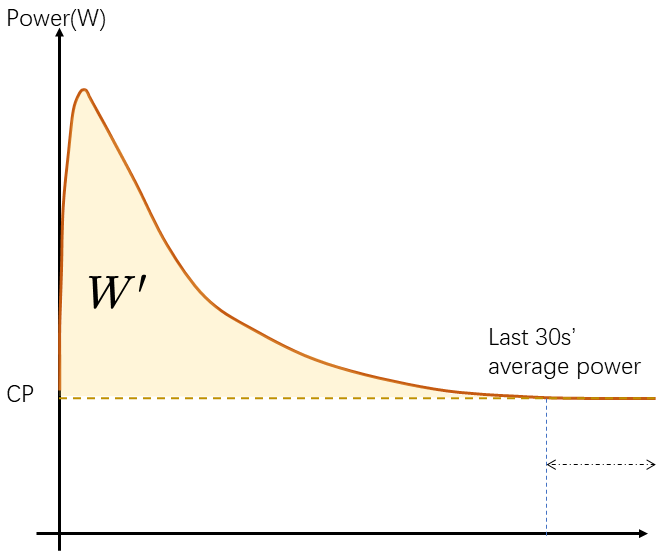
\includegraphics[width=6cm]{mcmthesis/figures/define of cp.png}
\caption{Measurement of ${W}'$ and CP} 
\end{figure}
In this problem, we compare the physiological indexes of several athletes and take this method as our parameter acquisition method.
\subsubsection{Energy Expenditure During Prolonged Exertion}
The two parameter (2-p) model\cite{morton_critical_2006} is a simple hyperbolic model. When an athlete's power output is higher than CP, the anaerobic energy ${W}'$ is continuously consumed to maintain this high power state. Therefore, the anaerobic energy consumed is $P-CP$. In a specified period, the maximum power an athlete can release is the power that can be achieved when all anaerobic energy is consumed. The 2-p model is given by:
%二参数模型
% 说明可以简成2参数模型  分析一下差异   在此问题中的适用性
\begin{equation}
    P(t)=\frac{W^\prime}{t}+CP
\end{equation}
\par
However, the 2-p model has a fatal defect, that in an extremely short period, athletes' power output can be infinite, which is unrealistic. Therefore, the three parameters (3-p) model \cite{morton_3-parameter_1996} is derived by translating the 2-p model shifted a certain distance to the left on the timeline. It is given by:
\begin{equation}
    t=\frac{W^\prime}{P(t)-CP}+\frac{W^\prime}{CP-P_{max}}
\end{equation}
\par
Inspired by the first law of thermodynamics and other natural phenomena, Puchowicz\cite{puchowicz_development_2020} raised the Omni Power Duration Model (OmPD), as a power curve based on exponential attenuation like this:
 %三参数模型
\begin{equation}
    P(t)=\frac{W^\prime}{t}\times(1-e^{-\frac{P_{max}-CP}{W^\prime}})+CP
\end{equation}
\par
We fit three different curves with the power data that top cyclists can produce at a given time, and the results show that OmPD model is the best. Therefore, in this problem, OmPD is adopted.
\begin{table}[H]
\centering
\begin{tabular}{llll}
\hline
  & 2-P    & 3-P    & OmPD   \\ \hline
$R^2$ & 0.9639 & 0.9996 & 0.9999 \\ \hline
\end{tabular}
\end{table}
It shows that the $R^2$ of each fitting curve is greater than 0.999, so the model is reasonable.
\begin{figure}[h]
	\centering  %图片全局居中
	\subfigbottomskip=2pt %两行子图之间的行间距
	\subfigcapskip=-5pt %设置子图与子标题之间的距离
	\subfigure[2-p model parameters]{
		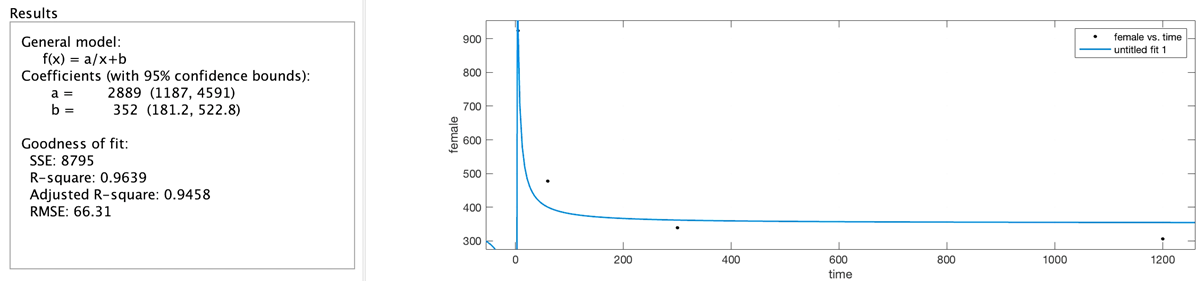
\includegraphics[width=0.70\linewidth]{mcmthesis/figures/p-2.png}}
		\\
	\subfigure[3-p model parameters]{
		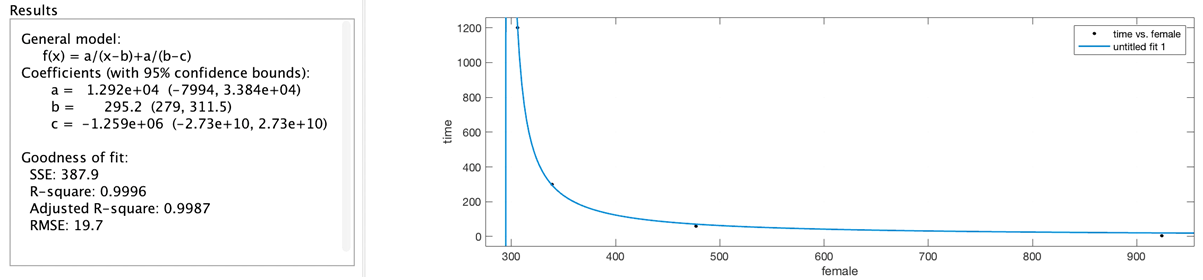
\includegraphics[width=0.70\linewidth]{mcmthesis/figures/p-3.png}}
	  \\
	\subfigure[OmPD model parameters]{
		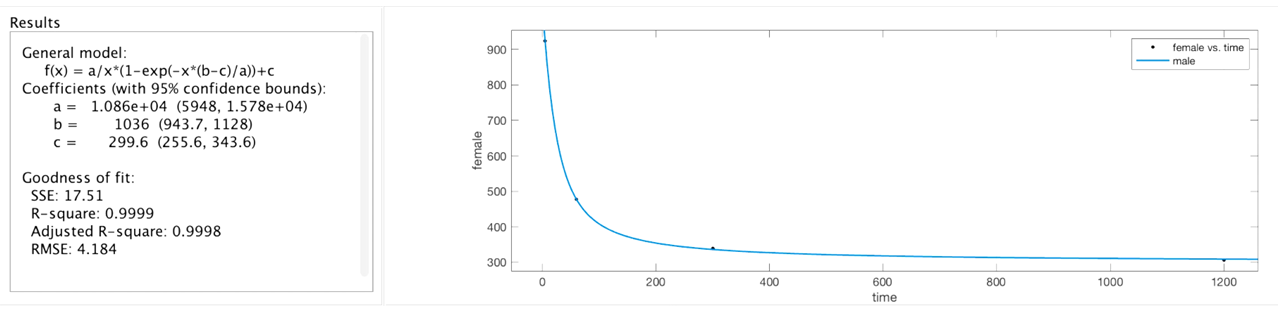
\includegraphics[width=0.70\linewidth]{mcmthesis/figures/para of woman.png}}
	%\quad
% 	\subfigure[fig4]{
% 		\includegraphics[width=0.48\linewidth]{./figs/4.png}}
	\caption{power model parameters}
\end{figure}
% \begin{figure}[H]
% \small
% \centering
% 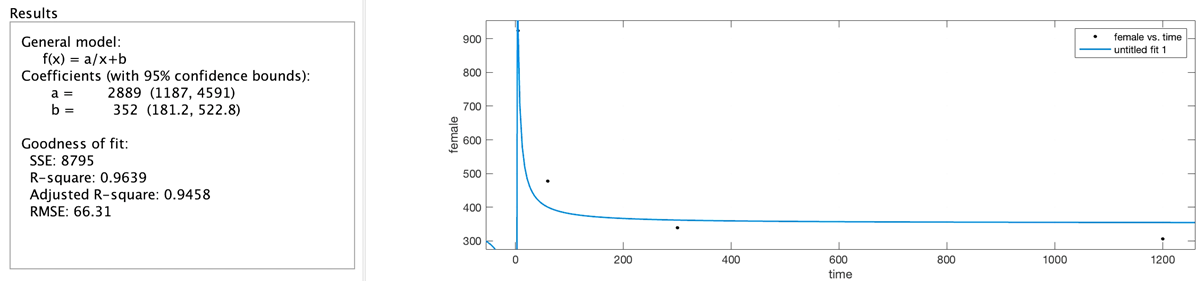
\includegraphics[width=14cm]{mcmthesis/figures/p-2.png}
% \caption{2-P} 
% \end{figure}

% \begin{figure}[H]
% \small
% \centering
% 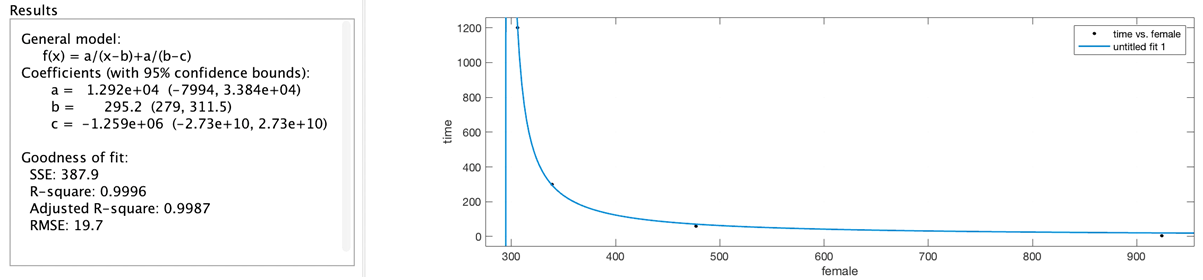
\includegraphics[width=14cm]{mcmthesis/figures/p-3.png}
% \caption{3-P} 
% \end{figure}

% \begin{figure}[H]
% \small
% \centering
% 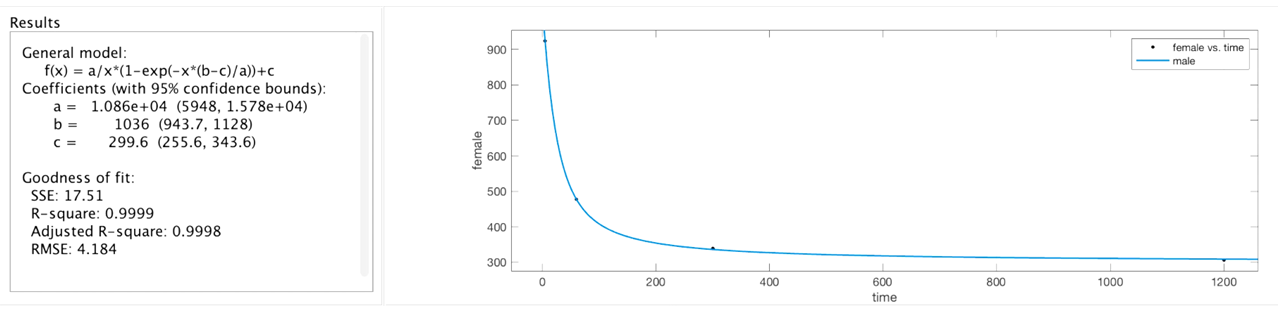
\includegraphics[width=14cm]{mcmthesis/figures/para of woman.png}
% \caption{OmPD} 
% \end{figure}


\subsubsection{Anaerobic Energy Expense and Recovery Model}
\par
The Available Anaerobic Work (AAW) is the anaerobic work that can be consumed by athletes under their current state, when athletes' output power is higher than CP, their remaining AAW will reduce. 
The exponential decay model-based power profile model has remarkable features that the output power won't be too large when $t$ is small, which indicates that the power used in its duration period will be more than the actual consumption of anaerobic work when it is close to $P_{max}$. Briefly speaking, when moving at a higher speed, the body will consume a greater part of the anaerobic work for heating and sweating, while the proportion converted into mechanical energy is lesser. Here we define a conversion coefficient that:
\begin{equation}
    \eta =P_{mechanical}/P_{consumed}
\end{equation}
\par
Reviewing OmPD's formula, we can find that $1-e^{-\frac{P_{max}-CP}{W'}}$ is equal to $\eta$. Therefore, AAW can be simplified into:
\begin{equation}
    AAW_{expense}=\int_{t1}^{t2}\frac{P}{1-e^{-\frac{P_{max}-CP}{W'}}}dt
\end{equation}
\begin{equation}
    AAW_{after}=AAW_{before}-AAW_{expense}
\end{equation}
\par
Similar to $W^\prime$ and CP, recovery ability is also an important standard to measure the level of an athlete. Here we use a One-Parameter Model to specify this, in which the parameter $R_a$ stands for athlete's recovery ability during aerobatic exercise. 
\begin{figure}[H]
\small
\centering
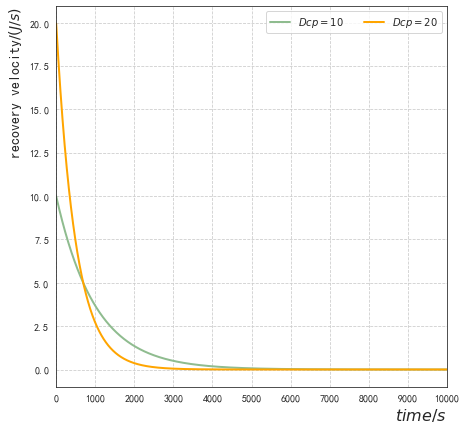
\includegraphics[width=9cm]{mcmthesis/figures/recovery -V.png}
\caption{Recovery speed} 
\label{fig:recovery}
\end{figure}
\begin{align}
    AAW_{after}&=W^\prime-[(P-CP)\cdot t] &, P& >CP\\
     AAW_{after}&=W^\prime-W^\prime_{exp}\cdot  e^{-R_a\cdot \frac{(CP-P)\cdot t}{W^\prime_0}} &, P& <CP
\end{align}
%插一张图, 固定t,Dcp 与恢复斜率之间的关系; 固定Dc p t与恢复总量的关系
\par
Figure \ref{fig:recovery} demonstrates the relation between anaerobic energy recovery velocity and time. Apparently, recovery velocity becomes quite slower as time goes, and when $D_{CP}(P-CP)$ becomes larger, recovery speed decreases much quicker. Therefore, the strategy for recovery is to seize the period when recovery velocity is quite large in one round.
% \subsubsection{Power Profile}
%%车手模型 
\subsection{Models of different types of riders}
Time trial specialists are the rider who has the all-around ability, therefore they can usually rank top in the time trial course. Compared with time trial specialists, climbers are better at medium power output and have poor burst output ability in a short time, so they have larger ${W}'$ and smaller $P_{max}$.
\par
The fitting results based on OmPD model are demonstrated in Figure \ref{fig:power output curve} and Table \ref{tab:different peple}(data comes from \cite{johnstone_how_nodate}):
\begin{table}[H]
\centering
% \tablename{the typical }
\caption{athletes' physiological ability} 
\begin{tabular}{llll}
\hline
                          & ${W}'$(J) & $P_{max}$(W) & CP(W) \\ \hline
Male time trial athlete   & 20790 & 1706    & 422.8 \\
Female time trial athlete & 10860 & 1036    & 299.6 \\
Male climber athlete      & 30880 & 1403    & 424.2   \\
Female climber athlete    & 18000 & 845.8   & 321.9   \\ \hline
\end{tabular}
\label{tab:different peple}
\end{table}
\begin{figure}[H]
\small
\centering
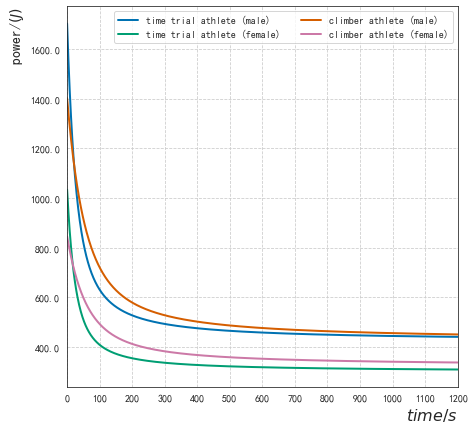
\includegraphics[width=8cm]{mcmthesis/figures/athlete-power-curve.png}
\caption{the power output curve of different athletes (expertise, gender)} 
\label{fig:power output curve}
\end{figure}
% \begin{figure}[H]
% \small
% \centering
% 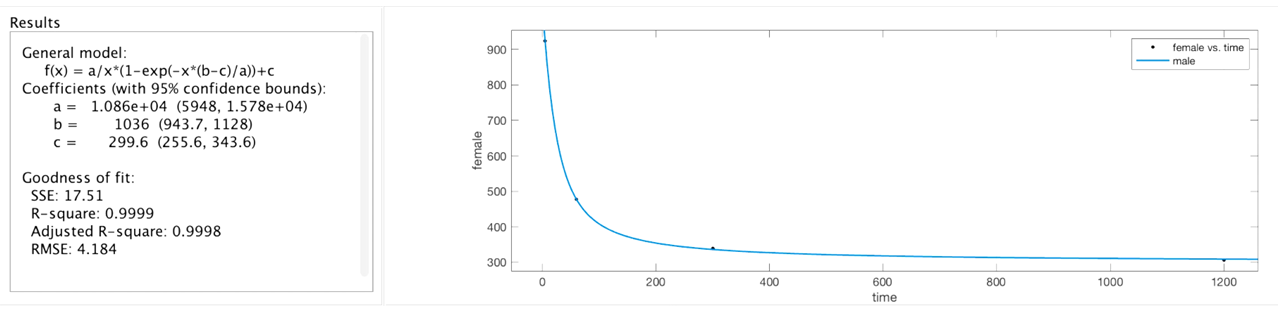
\includegraphics[width=14cm]{mcmthesis/figures/para of woman.png}
% \caption{Female time trial athlete} 
% \end{figure}

% \begin{figure}[H]
% \small
% \centering
% 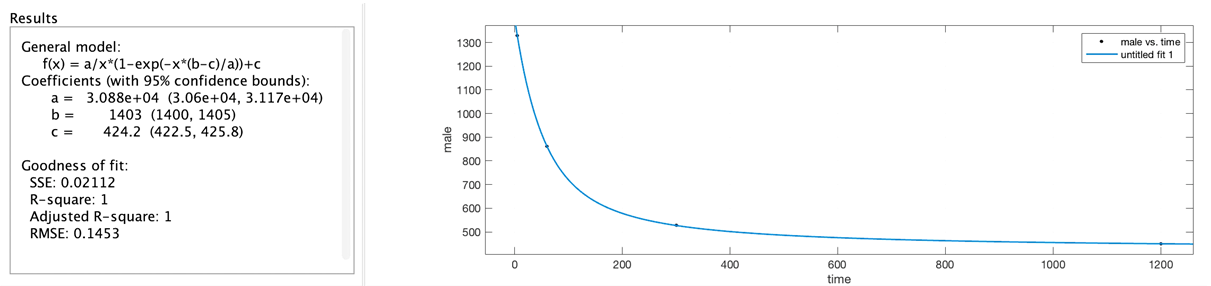
\includegraphics[width=14cm]{mcmthesis/figures/clamber-man.png}
% \caption{Male climber athlete} 
% \end{figure}

% \begin{figure}[H]
% \small
% \centering
% 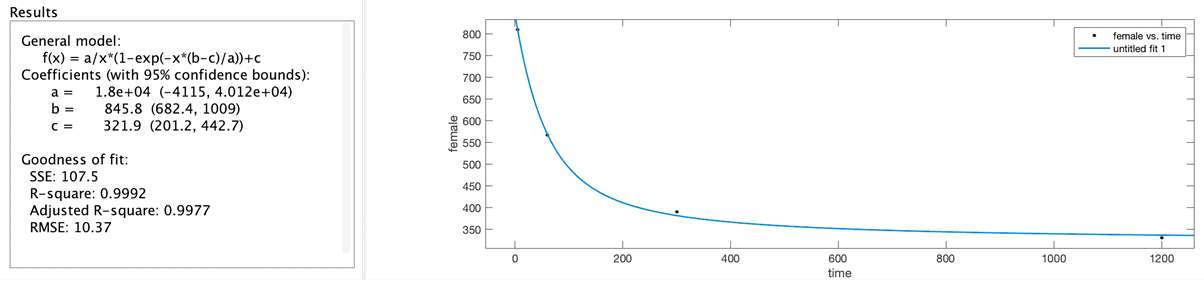
\includegraphics[width=14cm]{mcmthesis/figures/clamber-women.png}
% \caption{Female climber athlete} 
% \end{figure}

% \begin{itemize}
%     \item Note: a, b and c correspond to ${W}'$, $P_{max}$ and CP.
% \end{itemize}
\par

\subsection{Mechanical Model}
% It's necessary to make a physical model to get the relationship between output power and the velocity.
Here we established the model to correspond the mechanical model with the output power of the human body, the simplified schematic diagram of mechanical model is in Figure \ref{fig:Mechanical model}. This model not only include the impact of road undulation,  gravitational force. and friction, but also considered the external forces acting on the athlete like air resistance and so on.
\begin{figure}[h]
\small
\centering
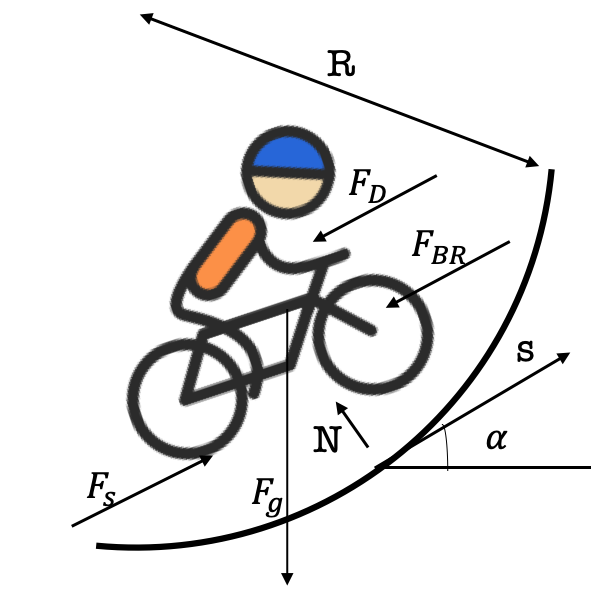
\includegraphics[width=4cm]{mcmthesis/figures/mechanical model.png}
\caption{Mechanical model} 
\label{fig:Mechanical model}
\end{figure}
\begin{align}
    F_s&=\frac{P_{bicycle}}{v}\\
    F_g&=m_{total}g\\
    F_D&=\frac{1}{2} C_DA\rho v^2\\
    f_1&=C_{rr}\cdot N\\
    f_2&=b_1+b_2\cdot v
\end{align}
\par
Where $C_{rr}$ is the rolling resistance coefficient, $b_1+b_2v$  is wheel bearing friction.
\begin{align}
    \dot{s}&=\sqrt{ \dot{x}^2+\dot{y}^2}\\
    \alpha&= tan^{-1}(\frac{dy}{dx})\\
    \frac{1}{R}&=\frac{y^{\prime\prime}}{[1+(y^\prime)^2]^{\frac{3}{2}}}
\end{align}
\par
Taking all the constraints listed above into consideration and simplifying, the following equation can be derived\cite{sundstrom_optimization_2013}: 
\begin{equation}
\begin{aligned}
    t^{\prime\prime}&= -(t^\prime)^4\frac{P_{bicycle}\cdot \eta_{tr}}{m_s}cos^2\alpha+t\prime \frac{(C_DA+A_w)\rho}{2\cdot m_s cos\alpha  }+t^\prime\frac{C_{rr}\cdot m_{tot}}{m_s}(g(t^\prime)^2cos^2\alpha+\frac{1}{Rcos\alpha})\\
    &+(t^\prime)^2\frac{b_1\cdot t^\prime \cdot cos\alpha +b_2}{m_s}+(t^\prime)^3\frac{m_{tot}\cdot g}{2\cdot m_s}sin2\alpha+t^\prime \frac{tan\alpha}{Rcos\alpha}
\end{aligned}
\label{equ:diff}
\end{equation}
\par
By introduce an auxiliary variable
to create a system of first-order ordinary differential equations, the equation\ref{equ:diff} can be solved with the Runge-Kutta Fehlberg method\cite{sreedhara_survey_2019}.
\par
When the bicycle turns, the athlete's body will tilt and the speed of the bicycle should not be too fast.
\begin{figure}[H]
\small
\centering
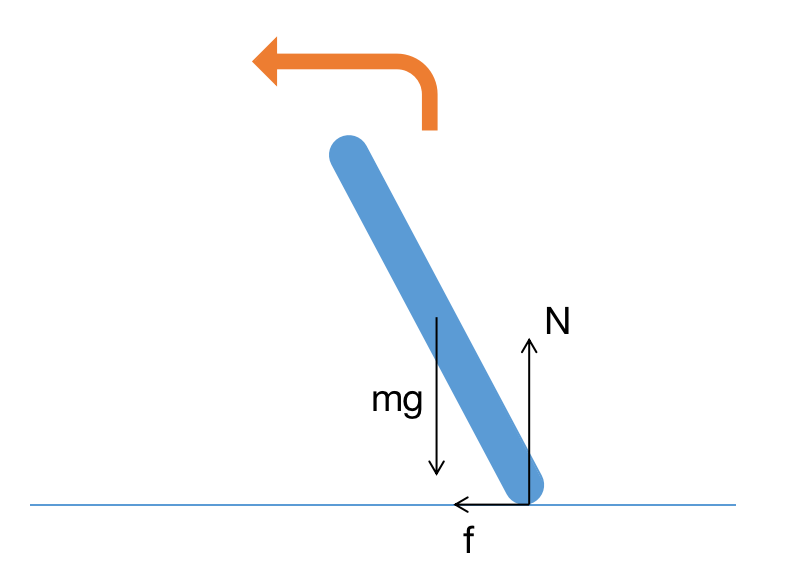
\includegraphics[width=4cm]{mcmthesis/figures/turn left.png}
\caption{schematic diagram when the athlete turns left} 
\end{figure}
\par
The following equation should be satisfied:
\begin{equation}
    f=\frac{v^2}{R}g
\end{equation}
\begin{equation}
    f\leq \mu mg
\end{equation}
\par
So, we have:
\begin{equation}
    v\leq \sqrt{\mu mR}
\end{equation}
\par
Where R is the radius of curvature of the curve.
\par
In addition, friction between bicycle chains and wheels is under consideration. These small resistances will lose mechanical energy, so the power obtained by the actual bicycle is:
\begin{equation}
    P_{bicycle}=P\cdot (1-loss)
\end{equation}


\subsection{Numeric optimization}
\par
We use sequential quadratic programming (SQP) for optimization, which can get the global optimal solution more effectively.
\par
The optimization problem is expressed as:
\begin{eqnarray*}
&& Minimize\ \ \ \ \ T=\sum_{1}^{k}\Delta t_i\\
&& subject\ \ to\ \ \ \ \ 0 \leq AAW_i \leq W'\ \ \ \ i=1,2,...k\\
&&\ \ \ \ \ \ \ \ \ \ \ \ \ \ \ \ \ \ \ \ \ \ P_{min} \leq P_i \leq P_{max}\ \ \ i=1,2,...k\\
&&\ \ \ \ \ \ \ \ \ \ \ \ \ \ \ \ \ \ \ \ \ \ \ 0 \leq v_i \leq v_{max}\ \ \ \ \ \ \ \ \ i=1,2,...k
\end{eqnarray*}


%%%section4
% \section{Tests of the Mathematical Model}

\section{Power Profile Model Results}
\par
Applying our models of cyclists to a different course, we get a shorter time to finish the course. We applied our model into the competitions below, 2021 Olympic Time Trial, 2021 Olympic Time Trial course and a course routine designed by ourselves. 
We obtained the map and altitude pictures on the official website of the race, used OpenCV for image processing, decomposed the track into pixel points, and made a linear difference between points to obtain the course data. The result are as follows.
% map
\begin{figure}[H]
	\centering  %图片全局居中
	\subfigbottomskip=2pt %两行子图之间的行间距
	\subfigcapskip=-5pt %设置子图与子标题之间的距离
	\subfigure[2021 Olympic Time Trial course routine]{
		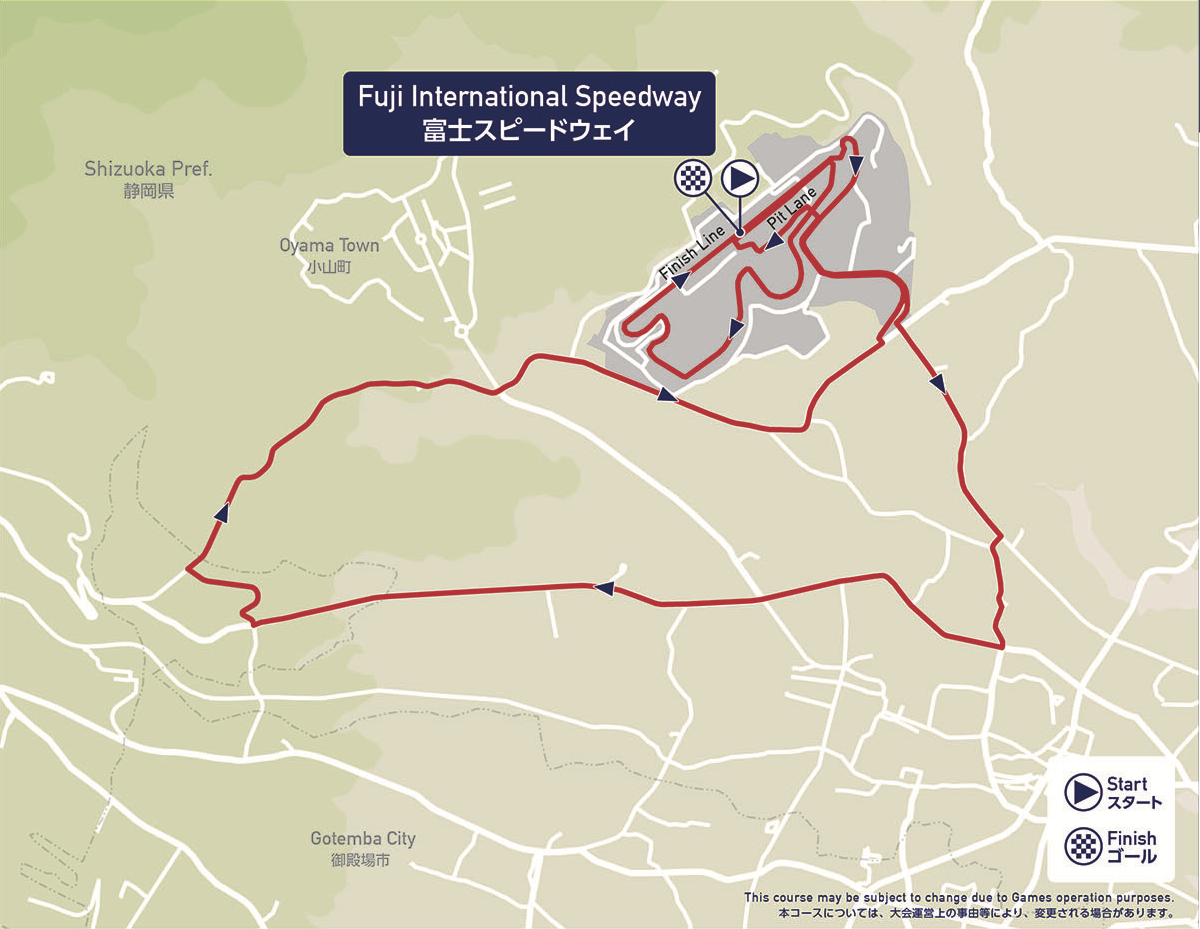
\includegraphics[width=0.48\linewidth,height=6cm]{mcmthesis/figures/jap.png}}
	\subfigure[2021 UCI time trial course routine]{
		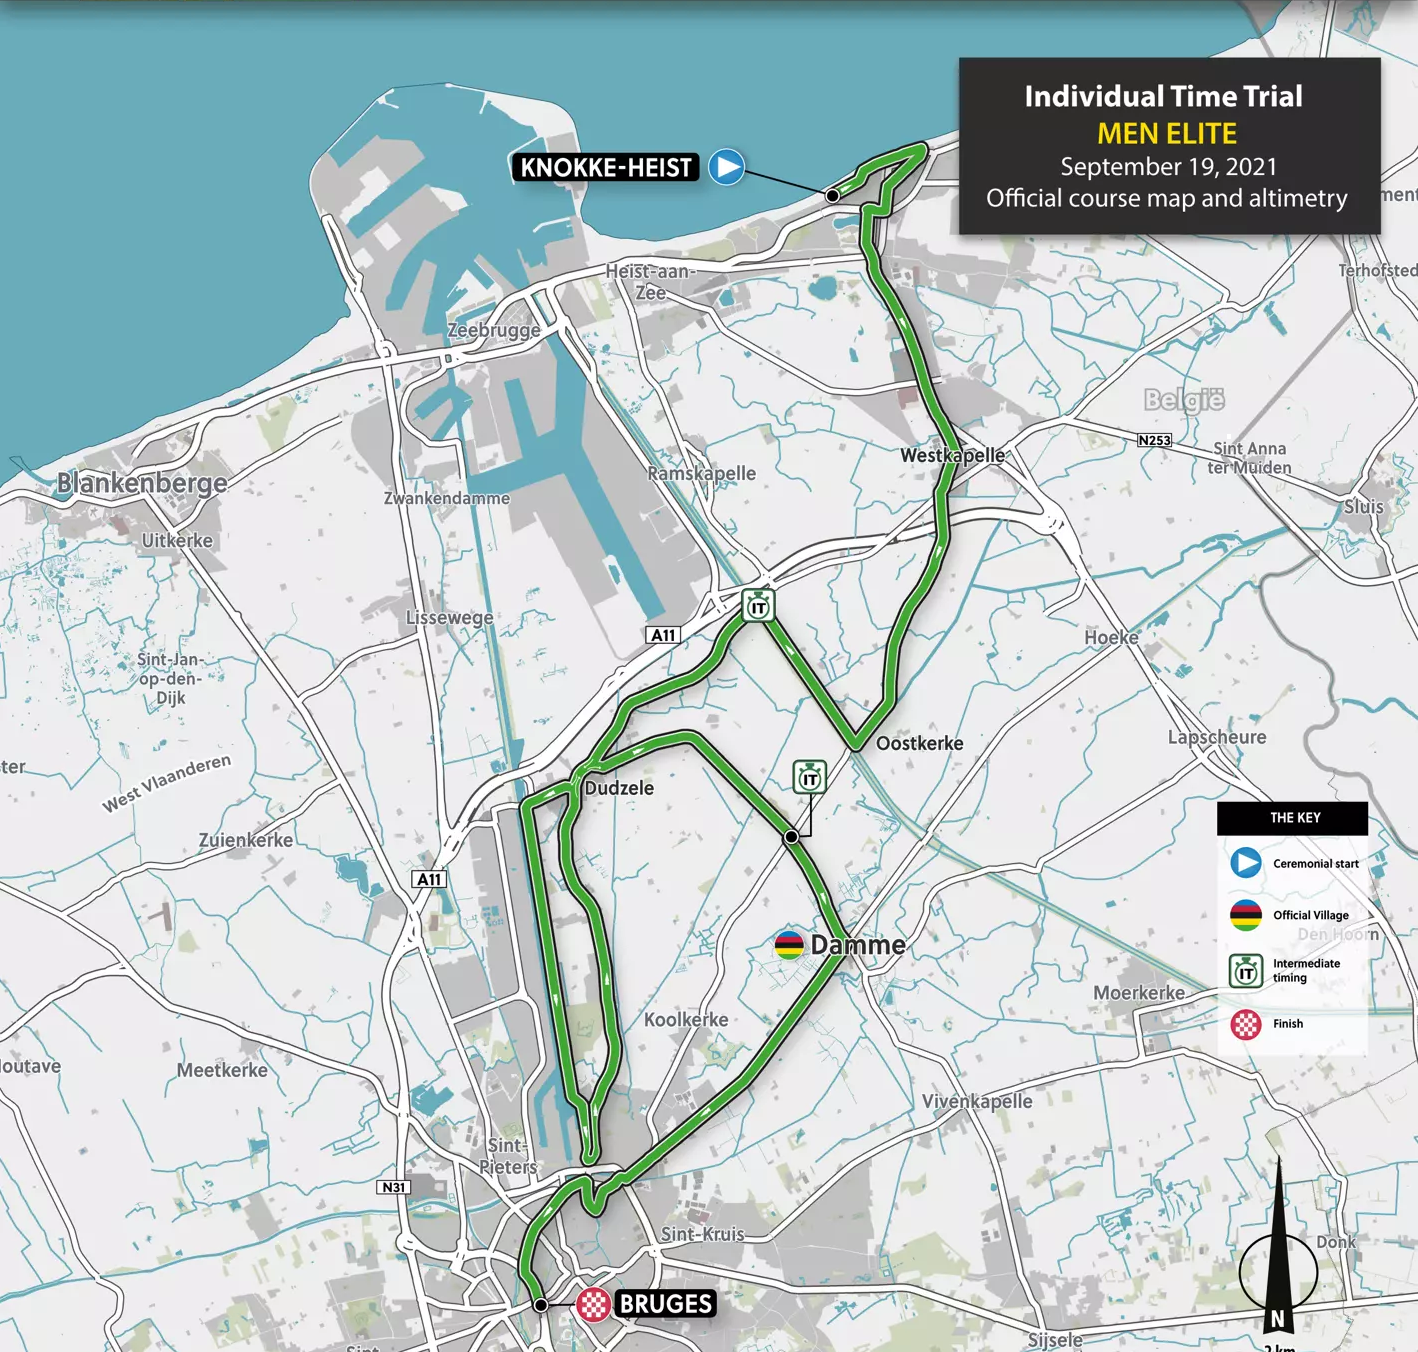
\includegraphics[width=0.48\linewidth,height=6cm]{mcmthesis/figures/bel.png}}
		\\
	\subfigure[altitude-distance change (man)]{
		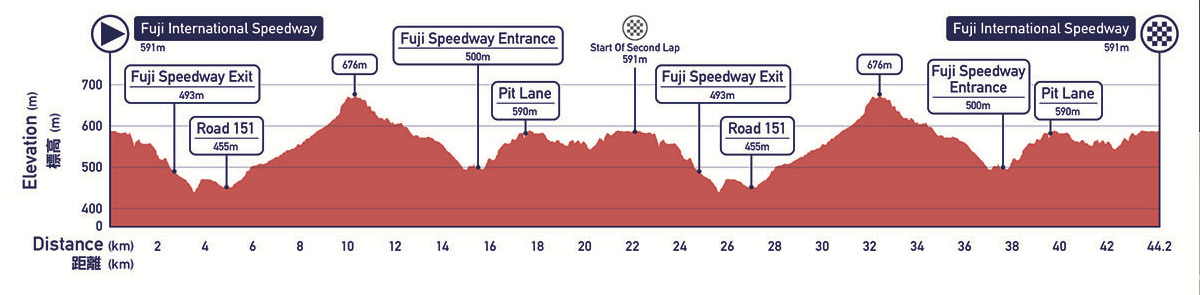
\includegraphics[width=0.48\linewidth,height=2.5cm]{mcmthesis/figures/jap-man.png}
% 		}
% 	\subfigure[2-p model parameters]{
		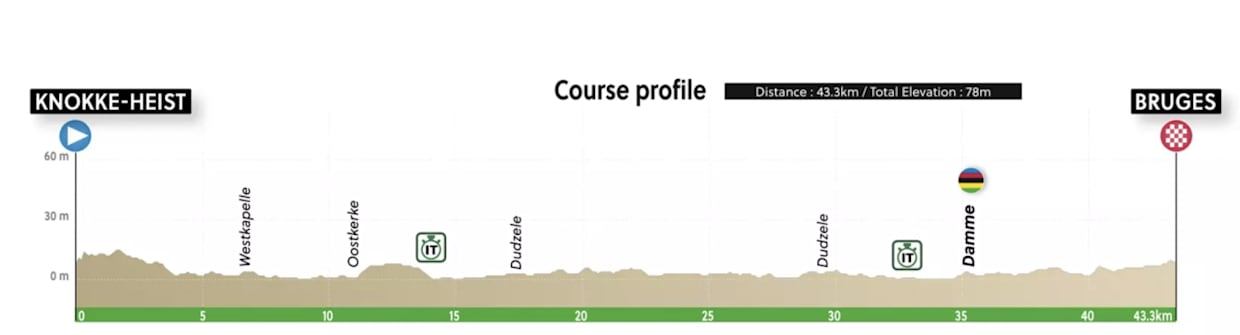
\includegraphics[width=0.48\linewidth,height=2.5cm]{mcmthesis/figures/bel-man.png}
		}
	  \\
	\subfigure[altitude-distance change (woman)]{
		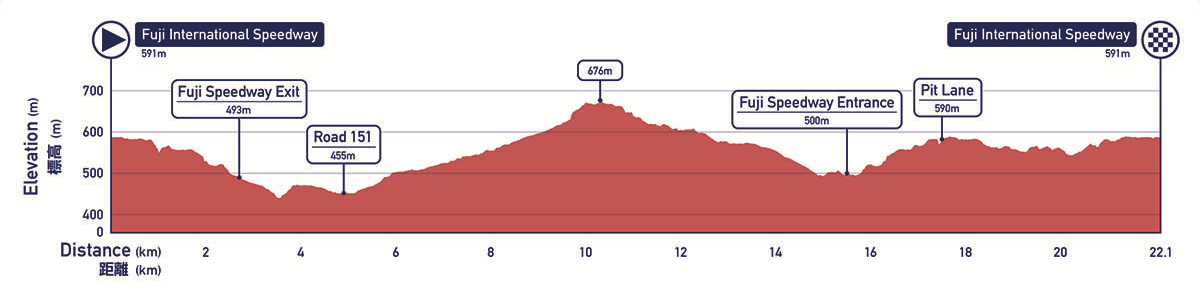
\includegraphics[width=0.48\linewidth,height=2.5cm]{mcmthesis/figures/jap-woman .png}
% 		}
% 	\subfigure[2-p model parameters]{
		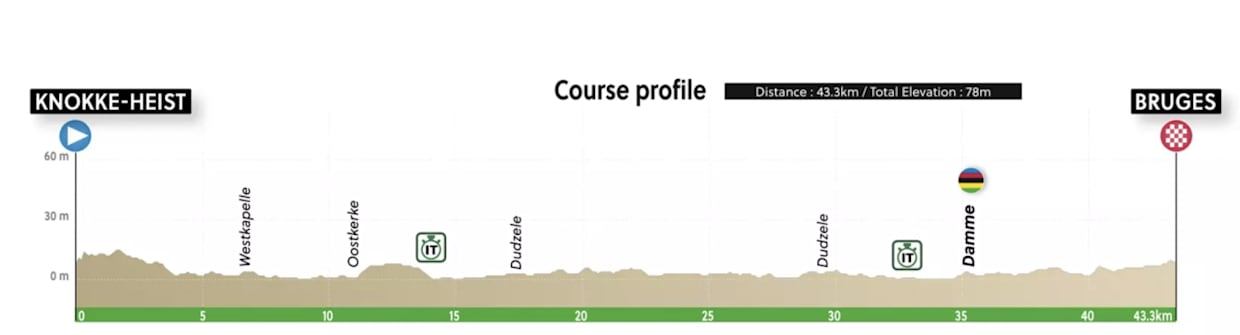
\includegraphics[width=0.48\linewidth,height=2.5cm]{mcmthesis/figures/bel-man.png}
		}
	%\quad
% 	\subfigure[fig4]{
% 		\includegraphics[width=0.48\linewidth]{./figs/4.png}}
	\caption{course information}
\end{figure}
\subsection{2021 Olympic Time Trial Tourse}
2021 Olympic Time Trial course was held in Tokyo, Japan, surrounding the Fujisan, the trial course has a large drop, it has higher requirements for athletes' long-distance output. Our model results points out that the output state of athletes presents a certain periodicity in the whole period. At the same time, the overall power output state and trend have a certain correlation with the change of altitude, this illustrates that the change of altitude is the main factor of athletes' output state, which is also consistent with our common sense.
% 日本  男 3105  女 1731  比利时  男2880 女 2154

\begin{figure}[H]
\small
\centering
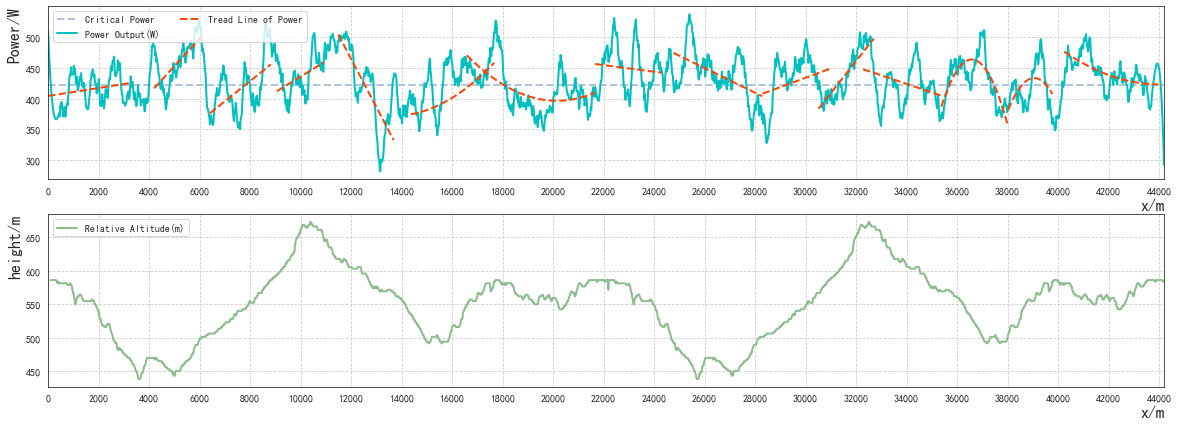
\includegraphics[width=13.5cm]{mcmthesis/figures/jap-m.png}
\caption{2021 Olympic Time Trial Tourse (male), finished in 3104.78s} 
\end{figure}


\begin{figure}[H]
\small
\centering
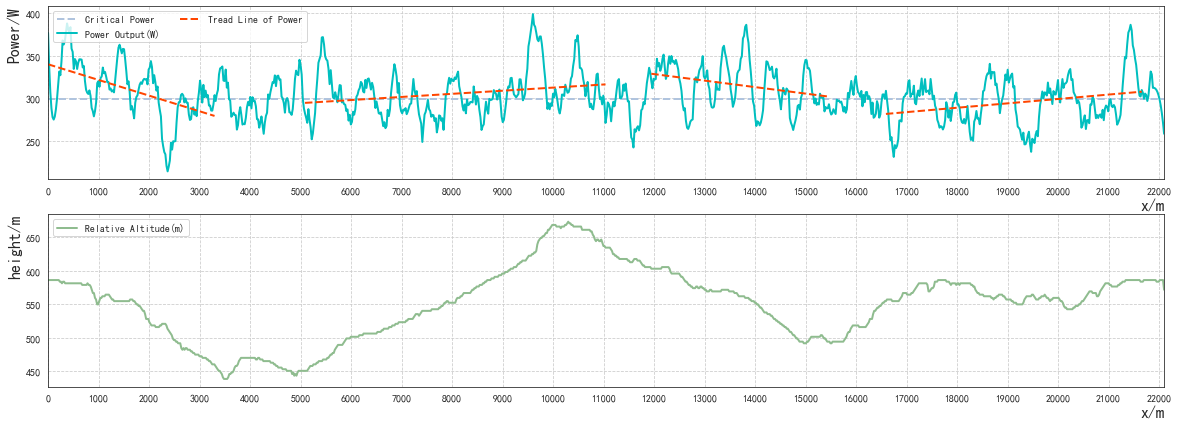
\includegraphics[width=13.5cm]{mcmthesis/figures/jap-w.png}
\caption{2021 Olympic Time Trial Tourse (female), finished in 1731.02s} 
\end{figure}


\subsection{2021 UCI World Championship Time Trial Course}
%map
The 2021 UCI World Championship Time Trial Course, on the other hand, was held on the highway, with a much smoother drop in altitude compared with that in Japan. The model results also shows a certain periodic changes, which is the same as the events held in Japan, and according with our experience.
\begin{figure}[H]
\small
\centering
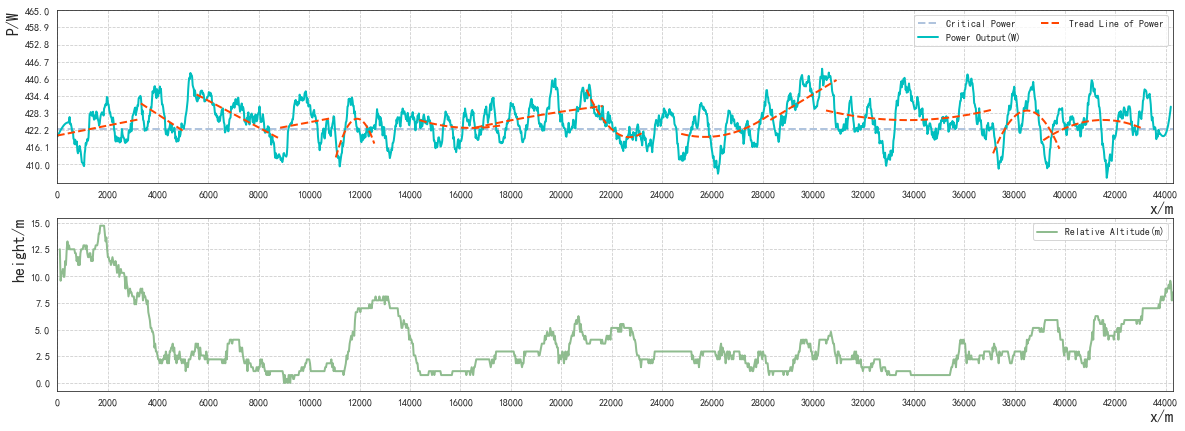
\includegraphics[width=13.5cm]{mcmthesis/figures/bel-m.png}
\caption{2021 UCI World Championship Time Trial Course (male), finished in 2880.23s} 
\end{figure}

\begin{figure}[H]
\small
\centering
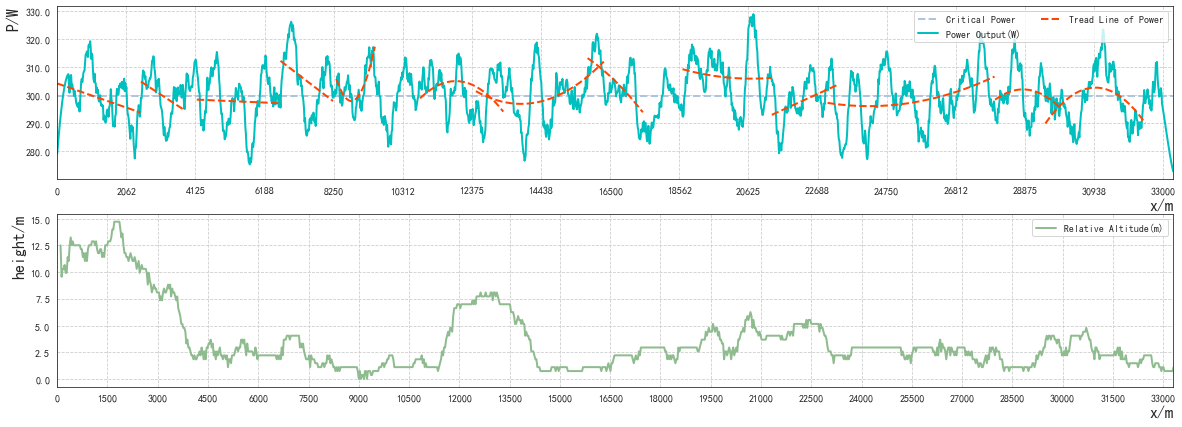
\includegraphics[width=13.5cm]{mcmthesis/figures/bel-w.png}
\caption{2021 UCI World Championship Time Trial Course (female), finished in 2154.79s} 
\end{figure}

\subsection{Our Course}
Follow the route of other competitions, we designed a simulated race line environment and applied our models, the results is like below. It also shows the periodicity in long period, also smoother than the previous results as the track and altitude changes are more gentle.
\begin{figure}[H]
\small
\centering
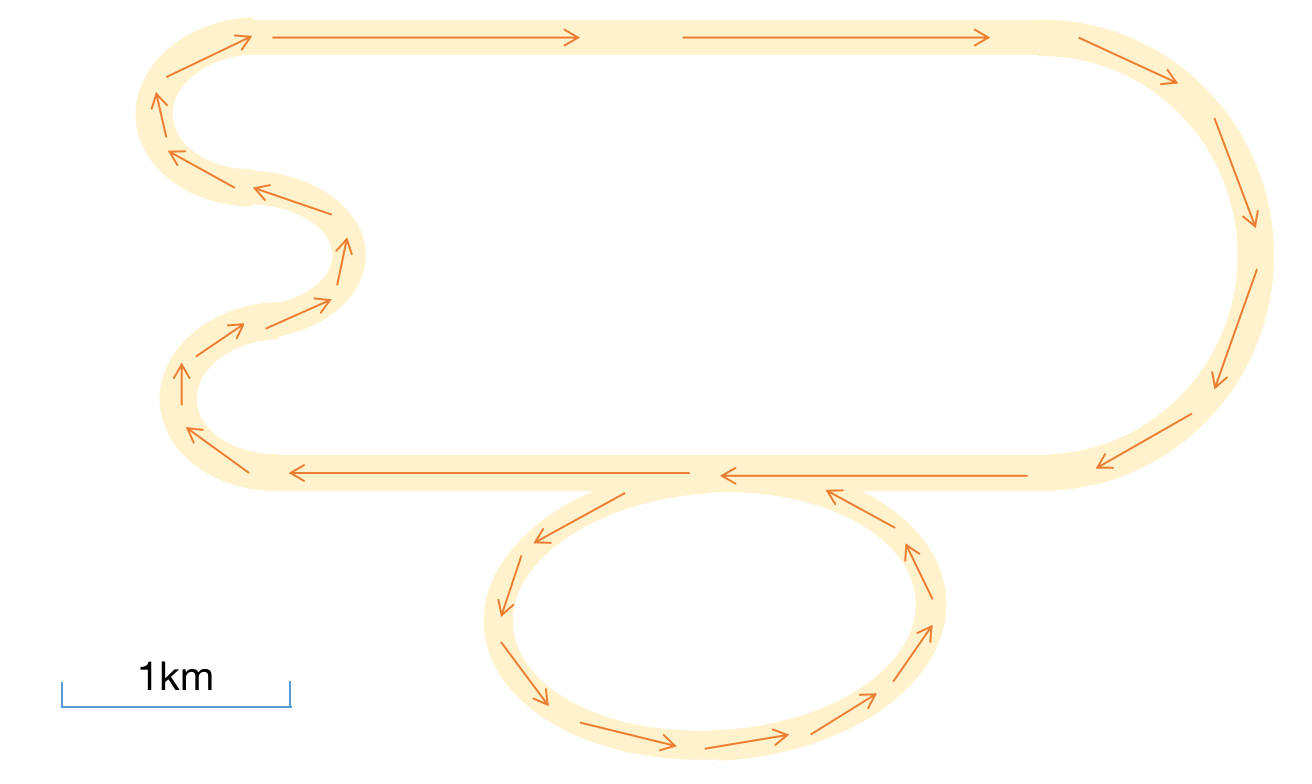
\includegraphics[width=8cm]{mcmthesis/figures/our course.png}
\caption{Course map} 
\end{figure}

\begin{figure}[H]
\small
\centering
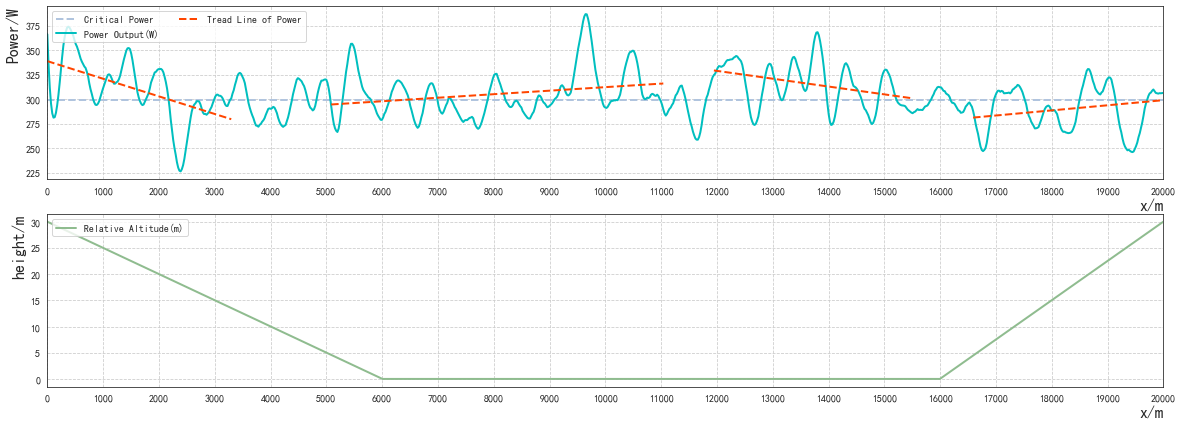
\includegraphics[width=13.5cm]{mcmthesis/figures/our.png}
\caption{The designed course (female) 1630.25s} 
\end{figure}
% 2020UCI 
% \subsection{Instructions}
% \subsection{Additional Instructions}
% \subsection{Additional Explanation}
% \par
% When solving practical problems, we simplify the model in the following aspects:
% \begin{itemize}
%     \item The inertia moment of the wheel has little effect on the work, and can offset each other during acceleration and deceleration, so it is ignored.
%     \item After calculation, $\eta$ is greater than 0.99 when p < 500 (for female time trial specialists), while there is little chance to achieve higher power in the actual competition. Therefore, the conversion coefficient is approximately 1 for calculation.
%     \item There is little difference between linear recovery and exponential recovery during energy recovery (between 0.95 to 1.05), so linear relationship is used during recovery.
%     \item We checked the competition data. Taking the Tokyo competition as an example, $\mu$ is 0.6, the road width is 11m, $m$ is 82.55. When turning 180 degrees, the turning radius is the road width at most. Therefore, the maximum value of $V$ is 23.34m/s, which is almost impossible for athletes in the competition. Therefore, the speed limit when turning is not considered.
% \end{itemize}


%%%section5
\section{Futher discussion}


\subsection{Sensitivity Analysis of Wind}
Without losing generality, we analyze the situation of the flat road. From the perspective of exercise physiology, it's easy to draw the conclusion that maintaining constant velocity saves energy. Thus, the cost of acceleration can be ignored in the long flat road, then the formula of P and v shows as below:
\begin{equation}
    P\Delta t=\frac{1}{2}m\cdot v^2+(b_1+b_2\cdot v+C_{rr}\cdot mg)\cdot \Delta l+k\cdot (v+v_{wind})^2\cdot \Delta l
\end{equation}
\par
First, we assume a map of 20km straightway with constant wind magnitude and direction.
The figure below depicts the relationship of the wind magnitude and final time of the same straight road. It's obvious that wind affects the final time to a large extent.
\begin{figure}[H]
\small
\centering
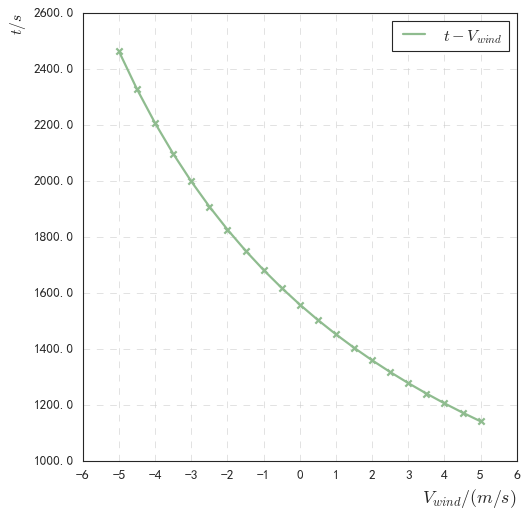
\includegraphics[width=6
cm]{mcmthesis/figures/t-wind.png}
\caption{Wind-final time} 
\end{figure}
Shown in the figure, the time result has an approximate quadratic relation with the magnitude of wind.

Second, sensitivity to the pacing strategy is analyzed. 
Usually, the magnitude of wind changes can't be predicted precisely during the process of the race, thus we can only give a vague strategy.

We assume another situation to simulate.
The map length is 20km because the race track is mostly circular, The wind direction to which the athletes are subjected is uncertain, they may be downwind for a period of time and upwind for another period of time. Wind during the front half is -5m/s (headwind), wind during the last half is +5m/s (tailwind). The athlete keeps a uniform velocity respectively in the front and last half. The figure below shows how the strategy affects final time. $P_{headwind}$ means output power in the front part suffering headwind.
\begin{figure}[H]
\small
\centering
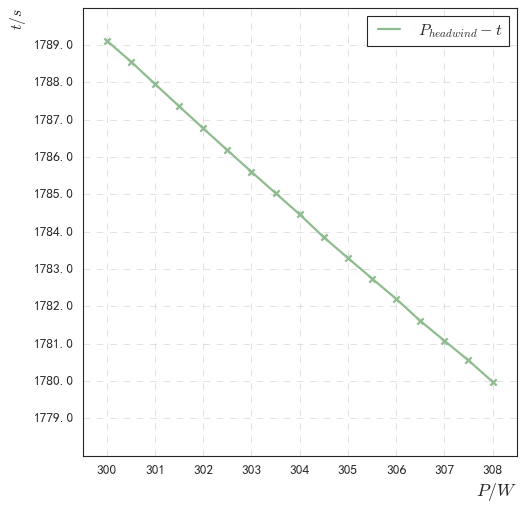
\includegraphics[width=6cm]{mcmthesis/figures/p-t-headwind.png}
\caption{P(headwind)-time} 
\end{figure}
From the figure, we can draw the conclusion that athletes should set power larger when confronting headwinds. But also, different strategy of anaerobic power distribution for the headwind and tailwind half only affects less than 10 seconds. Compared with the influence of slope, it affects little. Thus, the pacing strategy is not sensitive to wind variance.

%以平路为例来做,仅以CP为准来?
% 对常微分方程可以进行理论分析、稳定性分析etc
%风力变化-用时的图表,观察其中的关系
%风力变化-对总体的策略有无影响

\subsection{Sensitivity Analysis on Rider's Deviation}
In this part, we introduce the idea of a stochastic differential equation.

From the perspective of physiology, the rider can't control the output power precisely like a machine. It's inevitable to suffer deviations from the target power distribution. Because of the randomness of the deviation, we assume that the deviation follows a normal distribution.

To test the time-sensitivity, we give the front half output power a small perturbation:
\begin{equation}
    P_i=P_i+\sigma(i,t)P_i dB(\omega)
\end{equation}
where $\omega$ is individual sample points, $B(\omega)$ follows standard normal distribution. $\sigma$ stands for the degree of deviation, and here $\sigma$ is a constant.
We assume 4 types of deviation:
\begin{itemize}
    \item 1.always by CP\quad2.$\sigma = 0.01$\quad3.$\sigma = 0.05$\quad4.$\sigma = 0.1$\\
\end{itemize}
Then, optimize the rest half and get the result shown below.
\begin{table}[H]
\centering
\begin{tabular}{lll}
\hline 
Deviation Type    & final time(s) & increase in time(\%)\\
\hline
optimal strategty & 2793.52   & /    \\
1                 & 2853.44    &  2.14\% \\
2                 & 2837.95 &  1.57\%\\
3                 & 2861.39  &    2.43\% \\
4                 & 2910.36   &  4.18\% \\
\hline
\end{tabular}
\end{table}
The result shows even 1\% of normally distributed deviation causes more than 40 seconds time increase. Therefore, the strategy is sensitive to the strategy. Theoretical analysis, if the output power of the uphill section decreases, it'll cause increment to some extent. Thus, it's of necessity to stick to the strategy strictly.
\par
In addition, in the trial, it is difficult for athletes to change the power frequency quickly and in a large range. If it is divided into 100 points, athletes need to change the exercise power once in about 20 seconds for the Tokyo course. Therefore, we carry out smooth curve fitting on the optimization results, which is more in line with the sports law of athletes, so that athletes can better follow the optimization results.
\begin{figure}[H]
\small
\centering
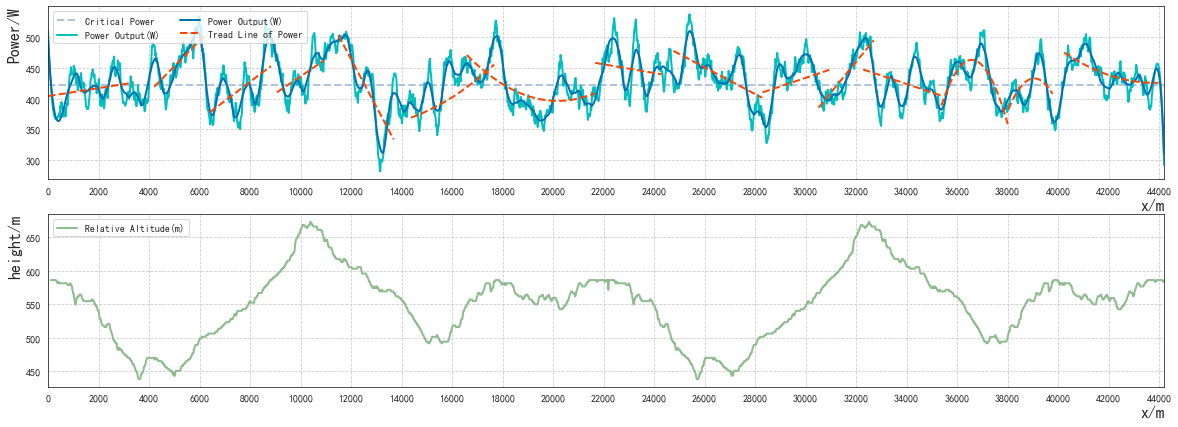
\includegraphics[width=13cm]{mcmthesis/figures/smooth.png}
\caption{Smooth curve of power for Tokyo course} 
\end{figure}

\subsection{Model in the Team Time Trial (TTT)}
\subsubsection{Aerodynamic Analysis}
\par The primary difference between the team time trial and individual time trial is in aerodynamics. the first rider overcomes the largest wind resistance while the drafting rides overcome smaller. Thus, the optimal strategy is based on drafting, where team members take the lead alternately, while others ride behind the leader, aiming to get more anaerobic energy totally by better recovery.
\par Taking both the reasonableness of spacing distance and the magnitude of the resistance into consideration, it's optimal to adopt the spacing d= 0.15m-0.5m. Then, according to the wind tunnel measurement and simulation by Bert Blocken\cite{blocken_aerodynamic_2018}, the relationship between position in the queue and the air resistance is depicted as follows:
\begin{figure}[H]
\small
\centering
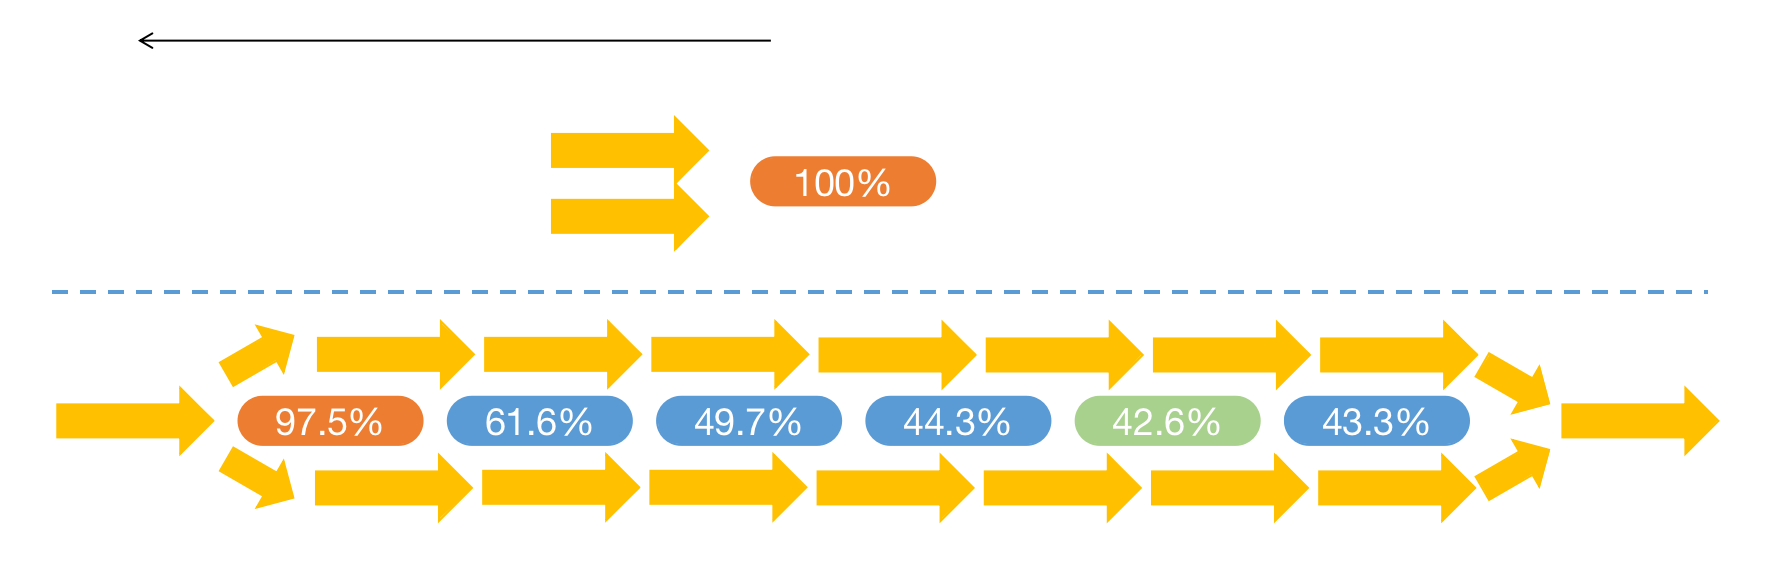
\includegraphics[width=12cm]{mcmthesis/figures/wind friction.png}
\caption{Air resistance in team compared to single person} 
\end{figure}
% 插入d=0.15 0.5 两张表格
\subsubsection{Model Adjustment}
\par
In our model, we take d = 0.15m and let the bicycle length (L$_{bicycle}$) = 1.8m. Thus, the length of a bicycle team is 11.55m. We can equivalently express the change of wind resistance at different positions by multiplying CdA by the corresponding coefficient.
\par
Considering the different physical abilities of each team member in the team, different W' and CP can be used to describe each athlete in the model. In this model, for convenience, athletes are divided into two groups of strong ability and weak ability, and they are sorted at the formation interval.
\begin{figure}[H]
\small
\centering
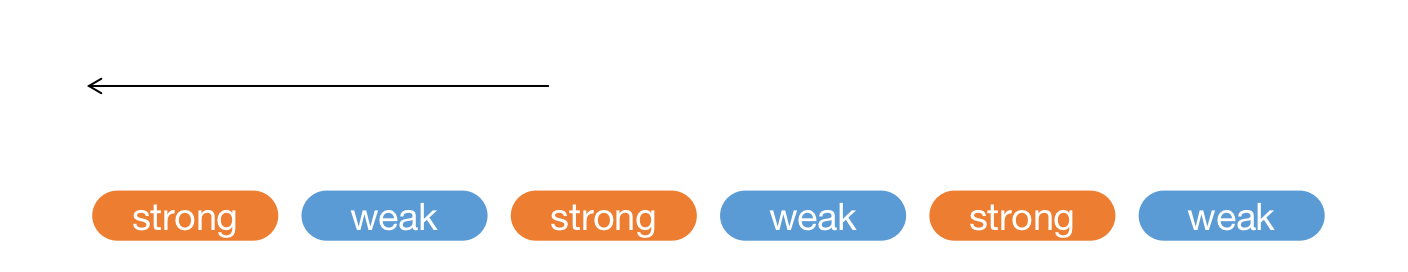
\includegraphics[width=14cm]{mcmthesis/figures/formation.png}
\caption{Formation} 
\end{figure}
\par
In the competition, the team speed is defined as V$_{team}$. Each athlete now consumes high power at the head of the team to maintain the team speed for a period of time, then decelerates back to the end of the team, and the teammates behind him step forward again against the wind. In this cycle, he can obtain a faster speed than when riding alone.

\begin{figure}[H]
\small
\centering
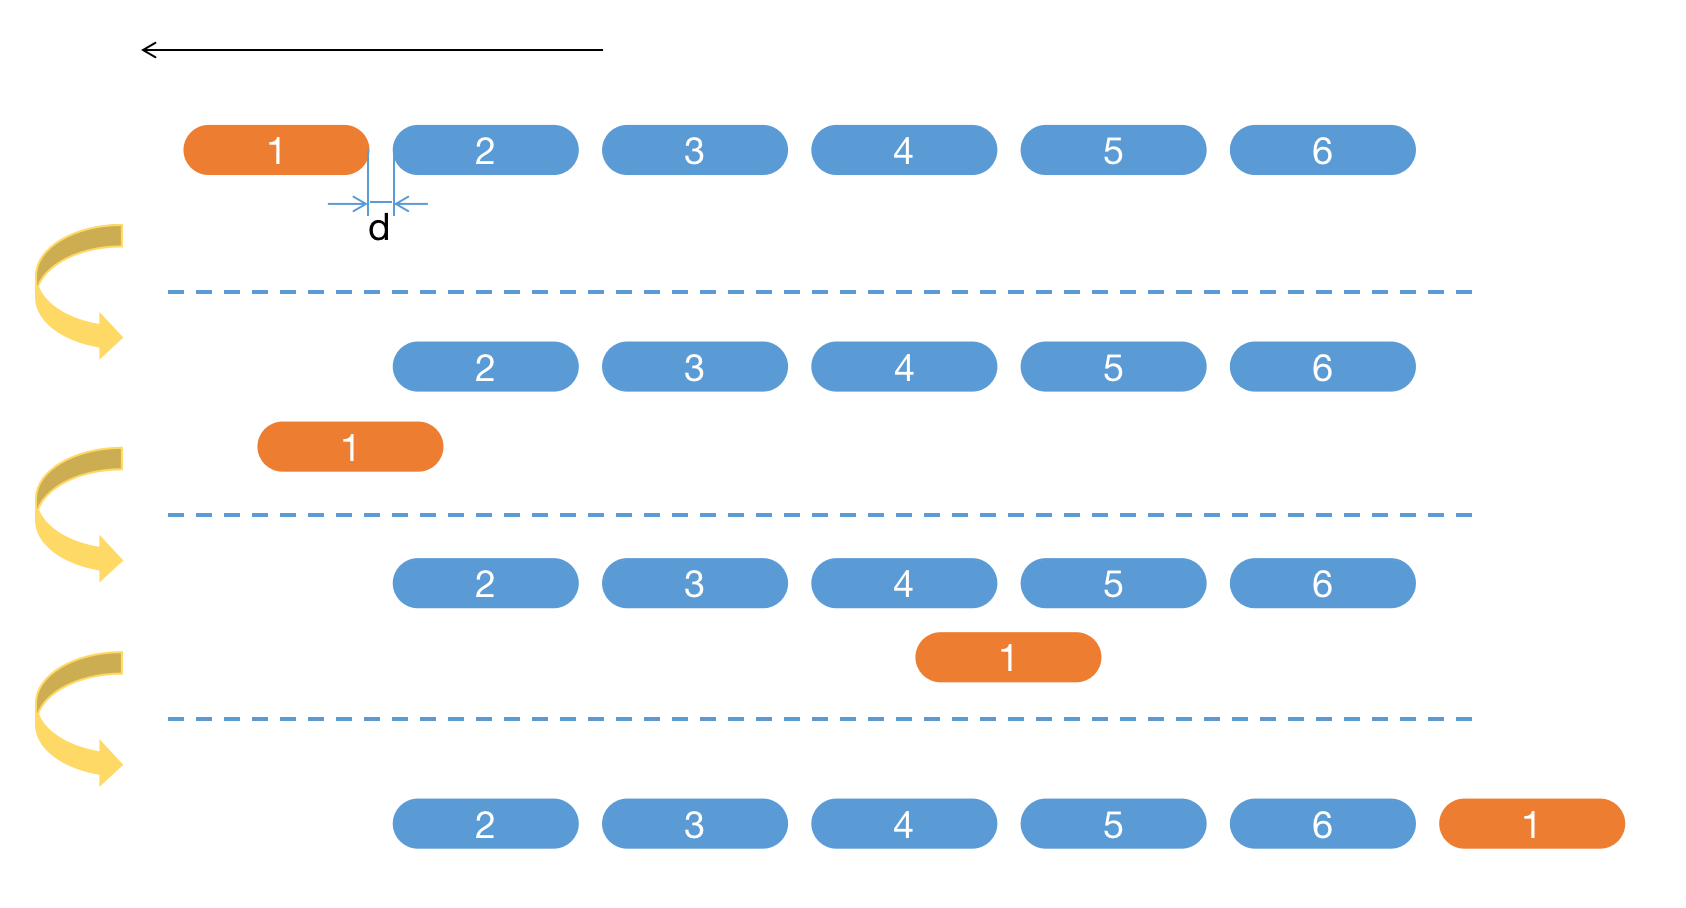
\includegraphics[width=14cm]{mcmthesis/figures/team change.png}
\caption{Formation transformation} 
\end{figure}

\par
Therefore, we can list the following equations according to kinematics.
Because it is moving at a uniform speed, it can be seen that:

\begin{equation}
k=\frac{1}{2}CdA\rho
\end{equation}
\begin{equation}
kv^2+mgC_{rr}cos\alpha+mgsin\alpha=\frac{P}{v}
\end{equation}
\par
We use k$_{i}$ (i=1,2...,6) to describe the different wind resistance at different positions. Thus, it shows:
\begin{equation}
P_{i}=k_{i}v_{team}^3+mgC_{rr}v_{team}cos\alpha+mgv_{team}sin\alpha(i=1,2...,6)
\end{equation}
\par
and
\begin{equation}
P_{back}=kv_{back}^3+mgC_{rr}v_{back}cos\alpha+mgv_{back}sin\alpha
\end{equation}
\par
It can be seen from the figure that returning from the head of the team to the tail of the team has traveled less $\Delta L$ than the whole team:
\begin{equation}
\Delta L=6\cdot (d+L_{bicycle})=(v_{team}-v_{back})\cdot t_{back}
\end{equation}
\par
In one cycle, we require that the available anaerobic work(AAW) consumed by the team member when facing the wind is equal to the anaerobic work recovered when following, that is, the change of anaerobic work in one cycle is equal to 0.
\begin{equation}
AAW_{expense}=AAW_{recovery}
\end{equation}
\par
At the same time, the value of AAW needs to be between 0 and W' in one cycle.
\begin{equation}
0\leq AAW\leq W'
\end{equation}
\par
In simultaneous equations (24) to (29), we can first assume that the windward time of a strong teammate (t$_{High}$) is the 20s, calculate the windward time and other parameters of a weak player, and finally test whether (30) is satisfied.
\par
The overall forward speed (V$_{straight}$) can be determined by the speed in the team (V$_{team}$) and the return speed (V$_{back}$).
\begin{equation}
v_{straight}=\frac{(3\cdot (t_{high}+t_{low})-t_{back})\cdot v_{team}+v_{back}t_{back}}{3\cdot (t_{high}+t_{low})}
\end{equation}
\par
We simulated riding on flat ground in MATLAB and found that using this strategy can increase the speed by 16.56\% compared with a single person riding.
\begin{table}[H]
\centering
\caption{speed comparision}
\begin{tabular}{lll}
\hline
           & single person & team work \\ \hline
speed(m/s) & 14.0274       & 16.3498   \\ \hline
\end{tabular}
\end{table}
\par
The obtained key parameters and AAW variation diagram are as follows:
\begin{table}[H]
\centering
\caption{key parameters}
\begin{tabular}{lllll}
\hline
t$_{high}$(s) & t$_{low}$(s) & v$_{team}$(m/s) & v$_{straight}$(m/s) & P$_{1}$(W)  \\ \hline
20       & 12.06   & 16.3498    & 16.3498        & 627.46 \\ \hline
\end{tabular}
\end{table}
\par
Where t$_{high}$ is the length of time a stronger teammate is at the head of the team, t$_{low}$ is the length of time a weaker teammate is at the head of the team.

\begin{figure}[H]
\small
\centering
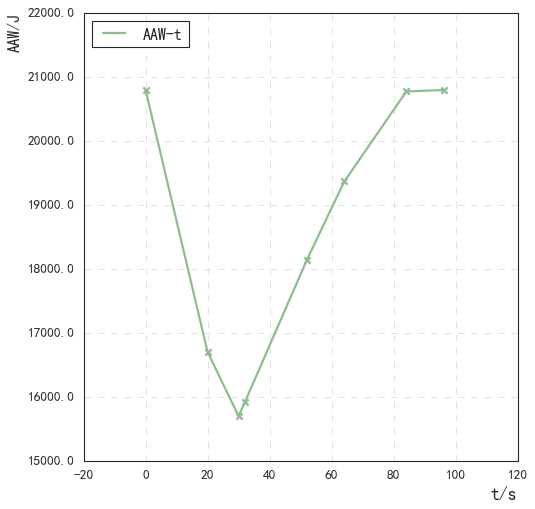
\includegraphics[width=8cm]{mcmthesis/figures/aaw-t.png}
\caption{AAW-t} 
\end{figure}

\par
It should be noted that when the wind direction changes, the bicycle fleet should adjust the direction accordingly.
\begin{figure}[H]
\small
\centering
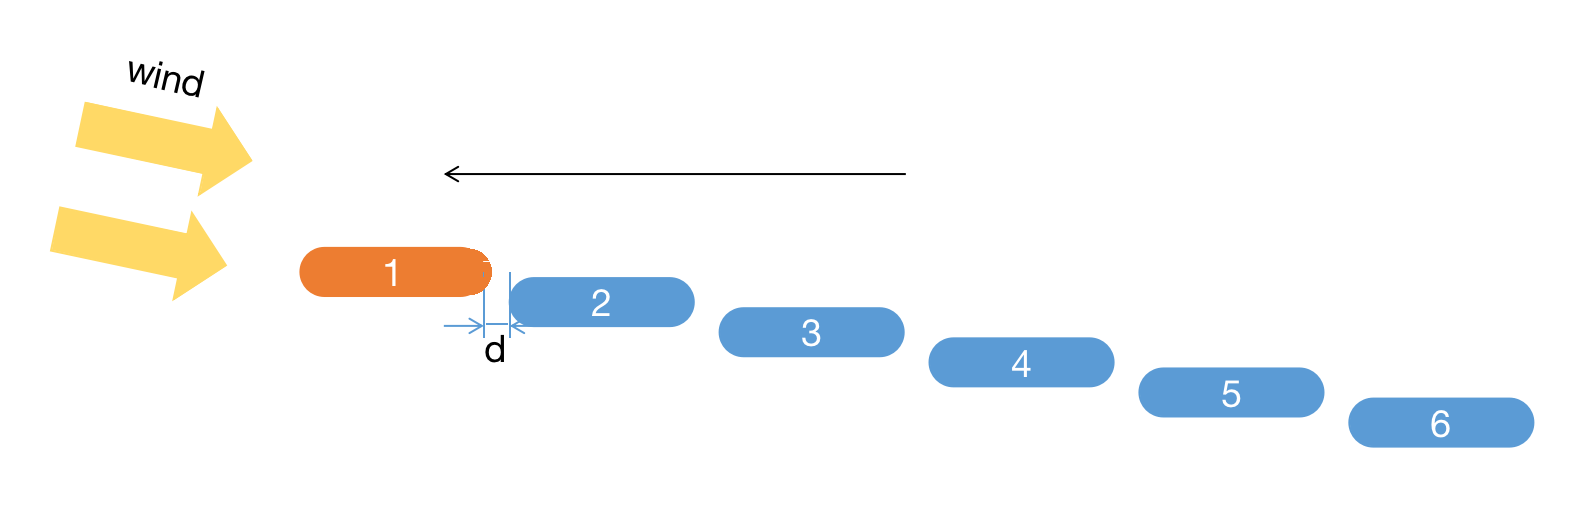
\includegraphics[width=10cm]{mcmthesis/figures/wind.png}
\caption{Formation in the wind} 
\end{figure}





% \begin{figure}[h]
% \small
% \centering
% 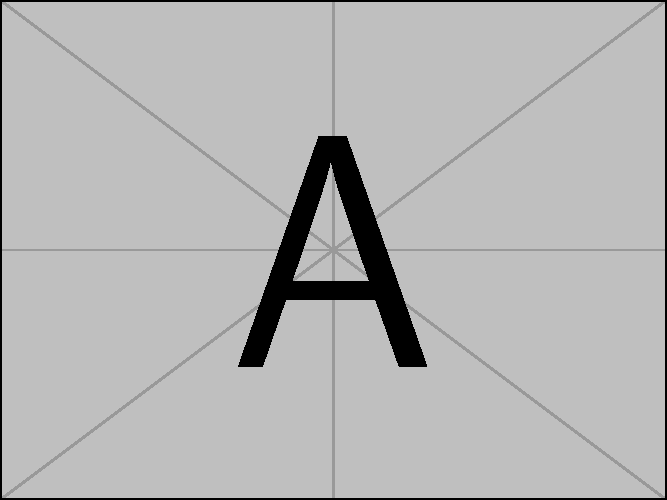
\includegraphics[width=8cm]{example-image-a}
% \caption{The name of figure} \label{fig:aa}
% \end{figure}


\section{Evaluate of the Model}

% \section{Strengths and Weaknesses}
% \lipsum[12]

\subsection{Strengths}
\begin{itemize}
\item \textbf{In line with human physiology}\\
According to the knowledge of human aerobic exercise and anaerobic exercise in biology, we establish our model through mechanism analysis. Facts have proved that our curve is in good agreement with the actual athletes. This makes our subsequent optimization more accurate.
\item \textbf{Faster in time trials}\\
By using our model and optimization algorithm, Top athletes can become faster. For example, in the Belgian women's course, the champion used 36min5s to finish. If she had used our model, she would have only used 35min 54s to finish. That's about ten seconds faster! 
\item \textbf{Easy for using and Wide application}\\
In practice, we only need to measure the relevant parameters of athletes with the 3MT method, input the course data and optimize with our algorithm, then we can get the optimal output power value at each time node. During the competition, the athlete is reminded to change the power through the software of real-time power measurement. This algorithm can be applied to different types of athletes and different courses.
\end{itemize}
\subsection{Weaknesses}
\begin{itemize}
\item \textbf{further discussion is not in perfection}\\
Due to time constraints, we only consider the situation on a small section of flat ground in our further discussion on the influence of the wind direction and the team time trial strategy. However, it is not difficult to transplant to uphill and downhill, and then you can combine them to get the strategy of the whole course.
\item \textbf{limits in actual operation}\\
In the actual race, athletes are required to output according to the set power. However, athletes cannot control their output power so accurately. Therefore, we smoothe the output power curve in further discussion (§4.2) to make it easier for athletes to realize and reduce errors.
\end{itemize}


\newpage
\section{Riders' Race Guidance via this Model}
\begin{spacing}{1.2}
%%行间距
\noindent \textbf{Energy consumption and recovery model}

An athlete's energy is divided into two parts, respectively for aerobic mechanism and anaerobic mechanism. There are three measurements – ${W}'$, CP, and $R_a$, to evaluate the athlete's capability.
${W}'$ is defined as a measurement of anaerobic work capacity.
CP, Critical power, is defined as the aerobic power level at which an athlete can keep the whole process of race, no matter how much anaerobic power has been consumed yet. 
$R_a$ is defined as an athlete's recovery ability.
AAW is the current anaerobic energy the athlete has, AAW (t=0) equals to ${W}'$.
When the output power is larger than CP, anaerobic energy is consumed, and AAW decreases. After AAW turns into 0, the output power cannot be larger than CP. On the contrary, when the output power is smaller than CP, anaerobic energy is in recovery, and AAW increases. Recovery speed depends on $R_a$.

\noindent \textbf{Measurement Methods of ${W}'$ and CP}

Athletes' daily strict training is aimed at improving these three measurements, to get a faster time in the time trial. Also, they need to have an accurate command of their capability to develop the strategy for the time trial.
3-min all-out test (3MT)  is highly recommended as the measurement method. During the test, the athlete is required to pedal at the all-out intensity with a dynamometer to measure, then draw the curve of time and power and derive the magnitude of ${W}'$ and CP as the figure shows.
\begin{figure}[H]
\small
\centering
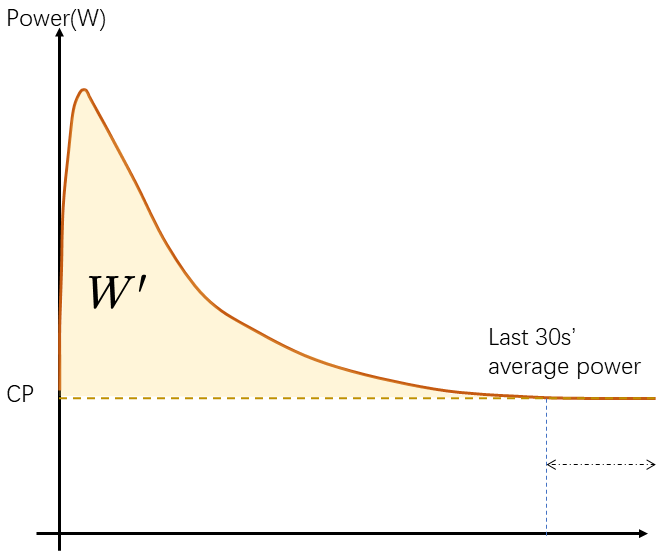
\includegraphics[width=8cm]{mcmthesis/figures/define of cp.png}
\caption{3MT result} 
\end{figure}
%%(P-t 3mt曲线图)
\noindent \textbf{Strategies for ITT riders}\\
1. Keep confident and positive all the time! Mood and mental state can affect the result to some extent. Also, moderate nervousness is quite normal, so don't worry. \\
2. Find your accurate magnitude of C, W', $R_a$ during daily training. Among these, the accuracy of CP influences most!  \\
3. Of course the best strategy is to follow the output power calculated by the algorithm we give. But if you can't remember and control the power precisely, then follow the vague strategy below, it's also of great help.\\
4. About slope: Set output power larger when you are going uphill, it influences much about your final time! The magnitude with which you can finish the whole up-slope is recommended. When going down-slope, you can decrease output power or even not step on the pedal if the down-slope is steep.\\
5. About wind: Set output power a litter lager when confronting a headwind. But it's not necessary to worry too much about the unpredictable wind condition, a different strategy for wind influences much less than the strategy for slope.\\
6. Don't be too fast before sharp turns, otherwise, you may be out of the circuit.

\noindent \textbf{Strategies for TTT}\\
1. The overall strategy in TTTs is based on drafting, where team members alternate in taking the lead, while others take advantage of the slipstream. When the leader's energy runs out, he will move away in a lateral direction and towards the back in the riding direction, allowing the second rider to take the lead.\\
2. The leading rider keeps a stable velocity that consumes his anaerobic energy out in one leading turn. The magnitude of velocity depends on the level of every member, and it needs to be decided cautiously.
\begin{figure}[H]
\small
\centering
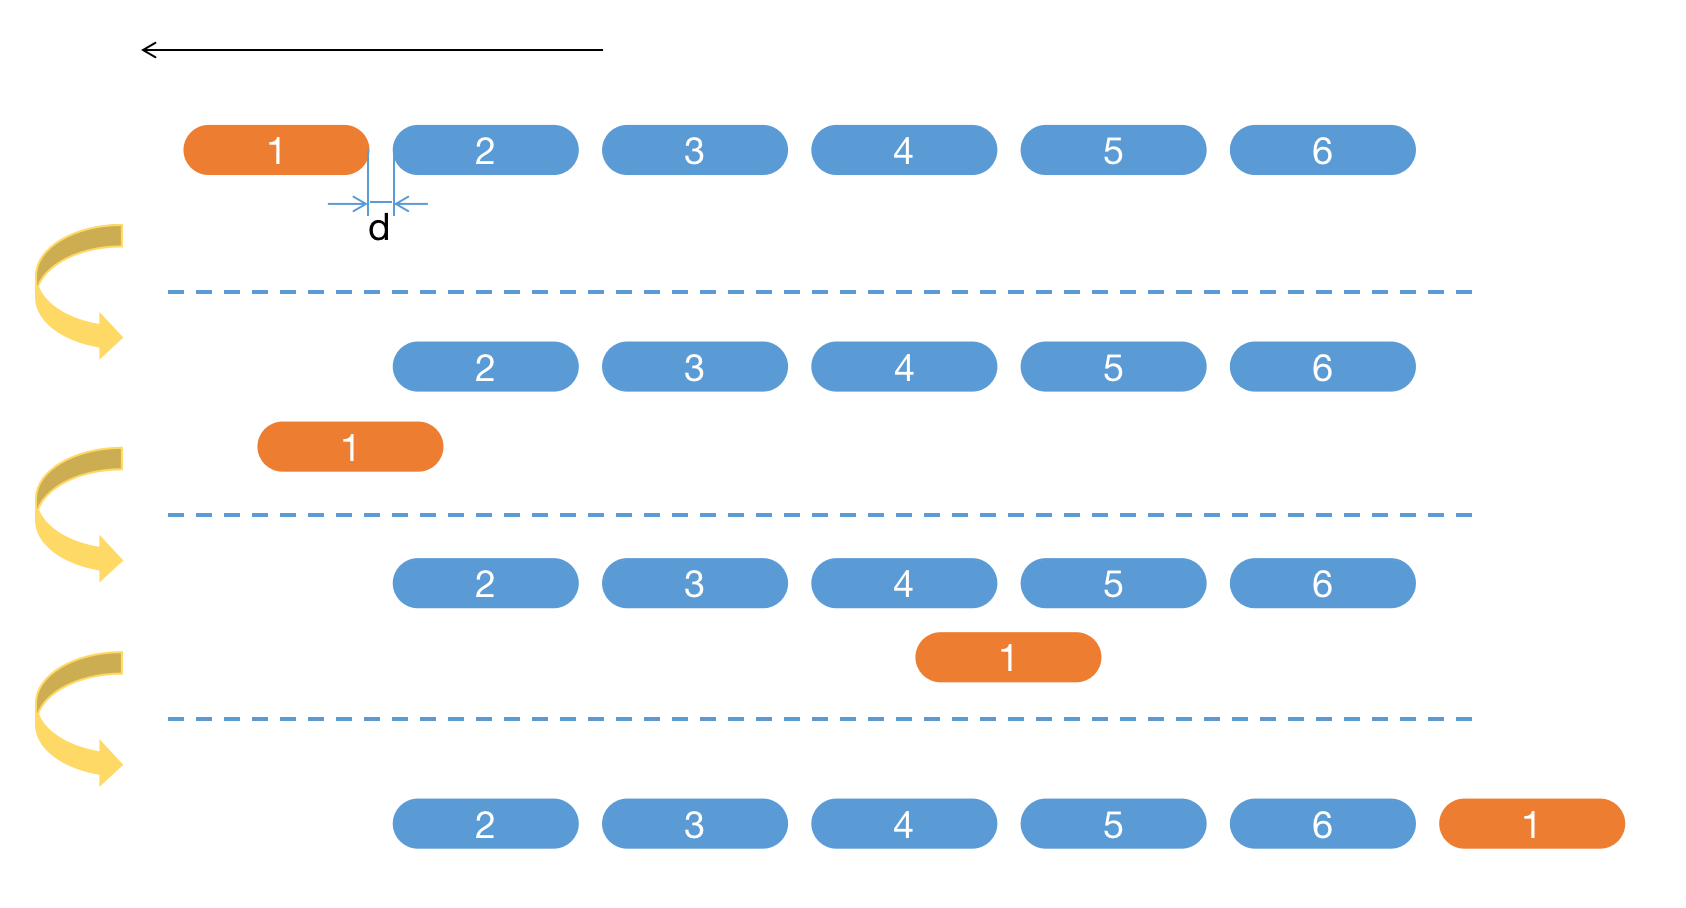
\includegraphics[width=8cm]{mcmthesis/figures/team change.png}
\caption{Formation transformation} 
\end{figure}
\noindent 3. Arrange strong riders and little weak riders alternately in the queue, and keep spacing between bicycles of 0.15 m-0.5m.\\
4. When the team is near the terminal, all the riders need to try their best to sprint, and no longer hold queues.

\end{spacing} 
\newpage
% \bibliographystyle{plainnat}
\bibliographystyle{IEEEtran}
\bibliography{22MCM.bib}

% \begin{thebibliography}{}
% % \bibitem{}
% \bibliography{bib.bib}
% \end{thebibliography}

% \begin{thebibliography}{99}
% \bibitem{1} D.~E. KNUTH   The \TeX{}book  the American
% Mathematical Society and Addison-Wesley
% Publishing Company , 1984-1986.
% \bibitem{2}Lamport, Leslie,  \LaTeX{}: `` A Document Preparation System '',
% Addison-Wesley Publishing Company, 1986.
% \bibitem{3}\url{https://www.latexstudio.net/}
% \bibitem{sreedhara_survey_2019}
% \end{thebibliography}
\newpage
\begin{appendices}
\noindent The simulation programmers used in our model are as follows.\\
\\
\textbf{1. optimization.m}
\lstinputlisting[language=Matlab]{code/T2_1.m}
\textbf{2. team.m}
\lstinputlisting[language=Matlab]{code/team.m}

% 日本  男 3105  女 1731  比利时  男2880 女 2154
% 

% some more text \textcolor[rgb]{0.98,0.00,0.00}{\textbf{Input C++ source:}}
% team\_fun.m
% \lstinputlisting[language=Matlab]{code/team_fun.m}

\end{appendices}
\end{document}
%% 
%% This work consists of these files mcmthesis.dtx,
%%                                   figures/ and
%%                                   code/,
%% and the derived files             mcmthesis.cls,
%%                                   mcmthesis-demo.tex,
%%                                   README,
%%                                   LICENSE,
%%                                   mcmthesis.pdf and
%%                                   mcmthesis-demo.pdf.
%%
%% End of file `mcmthesis-demo.tex'.
